% main_v2.tex — Simple Strategies in Information Ripples (v2 foundation draft)
% Scope: introduction, model, examples, on the one-axiom (mixed-anchor) foundation.
% Compile: pdflatex -> bibtex -> pdflatex x2, with the shared ref.bib.
% main.tex remains the full record (classification, computation, design); its
% results port to this foundation by redefining payoff rows for mixed anchors.
\documentclass[12pt]{article}
\usepackage[margin=1.1in]{geometry}
\usepackage{amsmath, amssymb, amsthm}
\usepackage{natbib}
\usepackage{booktabs}
\usepackage{setspace}
\usepackage{tikz}
\usepackage{float}
\onehalfspacing
\bibliographystyle{apalike}

\newtheorem{theorem}{Theorem}
\newtheorem{lemma}{Lemma}
\newtheorem{proposition}{Proposition}
\newtheorem{conjecture}{Conjecture}
\newtheorem{corollary}{Corollary}
\theoremstyle{definition}
\newtheorem{axiom}{Axiom}
\newtheorem{assumption}{Assumption}
\newtheorem{definition}{Definition}
\newtheorem{example}{Example}
\newtheorem{remark}{Remark}

% \mbox{}\\* forces the proof title onto its own line; rest is amsthm's own definition
\makeatletter
\renewenvironment{proof}[1][\proofname]{\par
  \pushQED{\qed}%
  \normalfont \topsep6\p@\@plus6\p@\relax
  \trivlist
  \item[\hskip\labelsep\itshape #1\@addpunct{.}]\mbox{}\\*
  \ignorespaces
}{%
  \popQED\endtrivlist\@endpefalse
}
\makeatother

\DeclareMathOperator*{\argmax}{arg\,max}

\title{Simple Strategies in Information Ripples}
\author{Li Quan\thanks{Faculty of Economics, University of Cambridge. Preliminary and incomplete working draft --- August 2026. Comments welcome. 
%This version rebuilds the foundation on a single axiom, with tied anchors resolved by uniform mixing rather than assumed away; it contains the introduction, the model, and the auction examples. Every numerical claim in the examples has been verified in exact rational arithmetic; the verification code is available from the author.
}}
\date{August 2026}

\begin{document}
\maketitle

\begin{abstract}
\noindent When nothing about opponents' beliefs is common knowledge, what can an analyst still predict? We study finite static mechanisms with symmetric payoffs and ordered private values, in which an agent weighs her action against an opponent's. \emph{Predictability} is the mass of types whose unique best action is the same under every centred perception of the opponent, measured under the analyst's benchmark distribution over opponent types, which neither agent need know. We give a finite test on the payoff table for predictability at a given benchmark; and a type has a unique prediction at every full-support benchmark exactly when one action weakly dominates its alternatives against each opponent type's conjectured play, strictly against at least one. Unpredictability has exactly two origins, and every tie between two actions is of one kind or the other: \emph{belief-driven} ties, which only exceptional perceptions sustain, and \emph{structural} ties, which the payoff rule imposes at every perception and every benchmark. Evaluating behaviour across subjective perceptions rather than at one commonly known distribution gives a partial, agents'-side answer to Wilson's robustness concern.
\end{abstract}

\section{Introduction}\label{sec:intro}

Equilibrium analysis is generous with its silences. In its standard pure-strategy form, a symmetric Bayes--Nash equilibrium in a sealed-bid auction, or a Cournot equilibrium in a linear-demand market, assigns each type exactly one action. Whatever variation shows up around that action in observed bidding or output data then has to be explained some other way: measurement error, unmodelled heterogeneity, or a departure from equilibrium reasoning severe enough to need a theory of its own. Unfortunately, none of these treats the width of the observed range as information in its own right; we lack an ex-ante prediction of which types should show a wide range and which a narrow one.

A Bayes--Nash prediction stands on two legs: each agent knows the distribution of opponents' private information commonly, and correctly forecasts the strategies they play. The simplicity literature has relaxed the forecasting leg, and in its dominance-based forms the distributional one too; what it keeps is the agent's question, whether she can find her optimal strategy, where this paper asks the analyst's. Dominant-strategy mechanisms, and the obviously strategy-proof mechanisms inside them \citep{li2017osp}, make both unnecessary, but the escape is narrow: most mechanisms of interest offer no dominant strategy, and where one exists the laboratory records persistent misplay \citep{kagel1987, kagel1993independent}. \citet{borgersli2019strategically} enlarge the class: strategic simplicity asks only own preferences, first-order beliefs about others' preferences, and others' rationality, never higher-order reasoning. Without a common prior the information leg fails first. An agent who knows neither its opponent's type nor its opponent's beliefs has no standard for a correct forecast, and no base on which to iterate reasoning about it: limited information is itself a limit on strategic sophistication. This paper relaxes the two legs together and asks what survives: \emph{for a given mechanism, which predictions hold however agents perceive their opponents, and which do not?}

Before any formalism, the idea fits in two auctions. Two bidders each may value an object at 1, 3, or 5. Sell it first-price, so the winner pays her own bid, with allowed bids 0, 1, and 2. The bidder whose value is 1 does best bidding 0 whatever she believes; the bidder whose value is 5 does best bidding 2 unless low-value opponents are very likely; the bidder whose value is 3 hesitates: bidding 1 is better against a low-value opponent, bidding 2 against a high-value one, and either belief is reasonable, so her action is unpredictable, and the unpredictability lives in belief. Now remove bid 2. With bids 0 and 1 only, every bidder has one best bid whatever she believes\footnote{Among the beliefs the model admits, which have full support: a bidder certain of facing one particular opponent bid may be indifferent.}: predictability rises from two-thirds at the uniform benchmark over the three values to one at every benchmark, bought by capping what can be bid. Sell the object second-price instead, so the winner pays the loser's bid (any whole bid from 0 to 5), and the value-3 bidder faces a different failure: against every opponent value in $\{1,3,5\}$, bids 2, 3, and 4 earn exactly the same. No anchored opponent is conjectured to bid in the gaps between the values, so the three outbid the same rivals and lose to the same ones; the single rival they sort differently is the one bidding 3, and beating him means paying 3 for a thing worth 3. No belief ranks the three bids, and refining the grid only multiplies the tied ones. Among grids that keep every value biddable, the one repair is alignment --- bids placed exactly at the values --- which collapses each bidder to a single action. It is also the demanding instrument: those values are the agents' perceived ones, so a designer must recover that perception from observed behaviour; the grid is a primitive here, and no choice of menu changes it. Belief-driven unpredictability responds to grid design; structural unpredictability, built by the payment rule, survives every grid that keeps each value biddable except the aligned one, and that exception is a knife-edge: one extra bid anywhere brings it back. That contrast is the paper: one measure, two origins, and a design lever for each, with sharply different reach.

The construction has three layers, and each is a conjecture the agent can actually form. First a \emph{reference}: knowing only which actions the mechanism allows, and nothing that distinguishes them, the agent treats them as equally likely. Second an \emph{anchor}: each possible opponent type is conjectured to play a best response to that reference, so the opponent's rationality enters without any hierarchy of beliefs, and where a type's best responses tie, the conjecture spreads weight over them equally. Third a \emph{centred belief}: the agent's own distribution over opponent types, free to tilt toward types near its own, the two sides tilted independently --- perceptions spreading outward from each type, the ripples of the title. The analyst's \emph{benchmark} is the yardstick against which that tilt is measured, and neither agent need know it. A belief and the anchors together give a conjecture over opponent actions, and the \emph{prediction set} of a type collects its best responses across every centred belief. A type is \emph{simple} when that set is a singleton and \emph{sensitive} otherwise, \emph{robustly simple} when it is simple at every benchmark, and \emph{predictability} is the benchmark mass of the simple types. The theory locates where perception matters, not which perception occurs. This gives a partial answer, on the agents' side, to the robustness concern of \citet{wilson1987}.

There is no fixed point on perceptions. Agents best respond to conjectured opponents and stop; imposing consistency would narrow prediction sets by assumption, and the range between the undistorted belief and near-total concentration on one's own type is precisely the object of interest. The uniform reference is also the standard first step of the level-$k$ literature, here derived from an axiom rather than posited, and measured reasoning depths concentrate at one to two steps \citep{nagel1995, arad2012, crawford2007levelk}. Iterating is open. The second-price (auction) ties below are ties against opponents conjectured to bid their values; allow opponents the bids the model itself predicts for them, with positive weight on each of the predicted bids, and those ties break. What survives at any depth is bidding one's own value: where every value is biddable it weakly dominates, so it answers every conjecture and lies in every prediction set the construction can produce.

One primitive should be said plainly before it is used. The type set is the set of opponents the agent can conceive, and it is coarse: a handful of possibilities rather than a continuum, and refining the bid grid does not refine it. Coarse processing of payoff-relevant quantities is well documented --- reasoning proceeds through a finite number of categories \citep{mss2008coarse}, opponents' contingencies are bundled into classes \citep{jehiel2005analogy}, probability judgements are compressed and noisy \citep{enke2023cognitive} --- and inside auctions too: in wholesale used-car auctions buyers read odometer readings by their leading digits, so prices fall discontinuously at ten-thousand-mile marks \citep{lacetera2012heuristic}. Financial markets show it too: quotes and trades cluster heavily on round prices even where a finer grid is available, and the price-resolution account of that clustering is that participants settle on a coarser set of values than the grid permits \citep{harris1991stock}. We take from that literature only its premise, that valuations are coarser than the price grid, and not its conclusions: where the \emph{mass} of orders sits is attributed there to negotiation and transaction costs, which this paper does not model and does not predict. That last concerns a good's characteristics rather than an opponent's type, but it is the same operation at large stakes. It also carries a warning for the design instruments below: buyers coarsen precisely where discriminating finely would gain them little, so a prediction that rests on a bidder preferring one bid to another by only a little is the kind least likely to survive contact with real bidders. The premise then does work rather than merely licensing a finite model. The gaps between perceived values are exactly where the second-price ties sit, so a bid grid finer than perception --- the ordinary case --- offers bids that no anchored opponent is conjectured to submit, and the framework predicts a range of bids around each value rather than truthful bidding. Those are statements about the conjecture, not prohibitions on observed behaviour: the framework predicts bids in the gaps. The persistent misplay noted above is therefore not evidence against the construction, although its direction is not something this paper speaks to. Alignment, which deletes those gaps, is correspondingly a knife-edge: only the exact match works, so the instrument asks for an exact match to a grid the designer never observes.

Three results make the split precise. A type's behaviour is pinned down at every benchmark exactly when one of its actions dominates every other against anchored opponents, and at a given benchmark exactly when the same comparison holds in weighted form; either way predictability is settled by finitely many sign comparisons and never by searching the beliefs themselves (Theorem \ref{th:dominance}). Every tie between two actions is either belief-driven or structural (Proposition \ref{th:sources}), which says how that dominance can fail. And a type is sensitive exactly when some centred belief makes two actions jointly optimal, and though those beliefs form a continuum, finitely many comparisons settle whether one does (Proposition \ref{prop:attainedtie}, Lemma \ref{lem:windows}). The auctions then separate the two origins and their design levers. In the second-price auction with every value biddable, sensitivity sits exactly in the gaps between perceived values (Corollary \ref{th:gaps}), and aligning bids to the values removes it (Corollary \ref{cor:align}), though no second-price grid keeping every value biddable gives a bidder any reason to prefer her predicted bid that survives every centred perception: the margin vanishes as her perception narrows to her own type, aligned or not (Corollary \ref{cor:spamargins}). In the first-price auction a two-bid cap is settled by a single sign condition (Corollary \ref{prop:cap}); where the possible values fall on both sides of the point at which the reference switches bids, that condition is an interval test --- full predictability at every benchmark exactly when no value lies just above the cap (Corollary \ref{cor:deadzone}). Section \ref{sec:model} sets out the model, Section \ref{sec:examples} the two auctions and the grid lever, Section \ref{sec:ties} the model's own tied anchors and the check against pure resolutions (Corollary \ref{cor:binary}), Section \ref{sec:literature} the literature, and Section \ref{sec:outlook} concludes.

\section{The model}\label{sec:model}

%(repetitive) The formal construction follows the same order as the economic argument. The mechanism fixes the action menu and payoffs. Neutrality supplies a reference over actions; rationality converts that reference into a type-specific anchor. A subjective belief then weights opponent types and, through their anchors, induces the action conjecture to which the agent best responds. Taking the union of those best responses produces the prediction set.

%\subsection{Primitives and the anchor}

There is a finite type space $T \subset \mathbb{R}$ and a finite action set $A \subset \mathbb{R}$.\footnote{Throughout, actions are denoted $b, b' \in A$, with $b''$ for a generic third action: in the leading auction applications actions are bids, and we keep the same letters in other applications rather than carry a second notation.} Two agents face a symmetric payoff $u(b, b'; t)$, where $b \in A$ is the agent's own action, $b' \in A$ the opponent's action, and $t \in T$ the agent's own type: values are private, in that the opponent's type does not enter the payoff, and interdependent values are outside this paper. Independence of the type draws is used only where revenue is computed and could be replaced by a joint-distributional benchmark over type pairs. A full-support benchmark distribution $p \in \Delta(T)$, with $p_s = p(\{s\}) > 0$ for every type $s \in T$, belongs to the analyst; throughout, $s$ denotes a generic opponent type in $T$. The benchmark is the yardstick against which subjective distortions are described. Agents need not know $p$. We read $p$ throughout as the composition of the opponent population. Shifting its weight across types is the comparative static the classification answers to. We assume $A$ contains no duplicate actions: distinct actions differ in payoff against some opponent action for some type, in at least one of the two roles.\footnote{This guards the uniform reference against redundant splitting of an action into copies, which would otherwise shift its weight. It keeps the reference well posed; no result below invokes it.}

The coarseness of $T$ is a premise: refining the physical value or bid grid does not refine $T$. One limitation is shared resolution: both agents perceive their opponents on the same grid $T$. Pooling agent-specific partitions does not restore generality: an agent perceiving only $\{1, 3\}$, of type 1, would want near-zero weight on type 2 but substantial weight on type 3, and weights that dip and recover violate centredness. So heterogeneous resolutions are outside the present model. Evidence for this coarseness is collected in Section \ref{sec:literature}.

%(Useful but overlap later) The informational setting explains why a reference exists at all. The mechanism --- the feasible actions and the payoff rule --- and the set of possible types are commonly observed; the distributional layer is not: agents share no prior over types, and an agent knows neither its opponent's type nor what its opponent believes. A conjecture about the opponent's action must start somewhere, and depth zero starts with no theory of the opponent's reasoning: conditioning on payoffs would already be such a theory, so the pre-strategic conjecture reads only the menu. That conjecture is the reference. Everything beyond it is subjective perception, admitted in a wide class rather than pinned by an equilibrium consistency requirement. The analyst, not the agents, holds the benchmark $p$ against which perceptions are described. In this sense the exercise gives a partial answer, on the agents' side, to the robustness concern of \citet{wilson1987}: predictions and designs are evaluated over a range of subjective perceptions rather than at one commonly known distribution.

The construction begins before strategic reasoning. Given only the feasible menu, the conjecturer forms a \emph{reference} $R_A \in \Delta(A)$ over the opponent's action: it knows which actions exist, but not what their labels or payoffs imply. Neutrality governs this first stage. Rationality enters only afterward: agents are risk-neutral expected-payoff maximisers. The first result is one line, and it fixes the starting point of the whole construction.

\begin{axiom}[Neutrality]\label{ax:neu}
A conjecture assigns equal weight to alternatives that the conjecturer's information cannot distinguish. In particular: (i) the reference belief, conditioning only on the feasible action set, is invariant to renaming: $R_A(\pi(b)) = R_A(b)$ for every permutation $\pi$ of $A$ and every $b \in A$; (ii) the conjecture over a type's tied best responses to the reference belief weighs the tied actions equally.
\end{axiom}

Clause (ii) becomes active only once best responses tie, a notion Definition \ref{def:anchor} makes precise below. With nothing left to distinguish the tied actions, the conjecture then spreads weight over them equally rather than favouring one.

\begin{proposition}[Uniform reference]\label{prop:reference}
Under Axiom \ref{ax:neu}(i), $R_A$ is the uniform distribution on $A$.\footnote{All proofs are in the Appendix.}
\end{proposition}

The proposition fixes the first stage. The second asks what each possible opponent type would optimally do against that uniform reference. Multiplying uniform expected payoff by $|A|$ does not change its maximisers, which gives the sum in the next definition.

\begin{definition}[Anchor]\label{def:anchor}
The \emph{reference best-response set} of type $t$ is
\[
B^0(t) = \argmax_{b \in A} \ \sum_{b' \in A} u(b, b'; t),
\]
the maximisers of expected payoff against the uniform reference. The \emph{anchor} $\beta(t)$ gives each action in $B^0(t)$ probability $1/|B^0(t)|$; when $B^0(t)$ is a singleton, the anchor is that action. When $|B^0(t)| \ge 2$ we call $B^0(t)$ a \emph{tied set}.
\end{definition}

Rationality narrows the conjecture to $B^0(t)$. If that set contains several actions, the available information says nothing further about which one is chosen, so clause (ii) assigns them equal weight. The anchor mixture records the conjecturer's unresolved uncertainty. It is not a claim that the opponent randomises in observed behaviour.\footnote{Hierarchical models impose point-valued conjectures at every level by convention: level-$k$ from a uniform level-0 \citep{nagel1995, stahl1995, crawford2007levelk}, cognitive hierarchy from a mixture of lower levels \citep{camerer2004cognitive}. The kinship is with the first step only: our uniform reference coincides with the level-$k$ starting point, here derived from the axiom rather than posited; cognitive hierarchy's mixture over lower levels is a different convention, not a special case of ours. A type is a cell of the agent's partition of opponents, one behaviour per cell \citep[compare][]{jehiel2005analogy}.}

%(Useful but too early) The second clause is audited, not trusted. Fix the ties: a \emph{resolution} picks one action from each tied set, generates its own rows, and yields its own prediction sets; the union of these across all resolutions is the \emph{scenario benchmark} --- the forecast of an analyst whose agents somehow know how ties resolve. The model's prediction and the benchmark are related exactly in Appendix \ref{app:resolutions}: a predicted action is, against each competitor separately, unbeaten under some resolution at the same belief; with two actions the prediction is contained in the benchmark; in general the two part in both directions, and the parting is economics --- the benchmark keeps scenario specialists that the conjecture drops, while the conjecture can predict a hedge across the tie that no single scenario supports. Hedging is what rational ignorance looks like, and the premise of the model is that the resolution is not knowable; where the objects differ, both are reported. In the tied instance of Section \ref{sec:tied} they coincide, and the coincidence is a theorem rather than luck: the action set there is binary. In the second-price application the question does not arise: truthful bidding weakly dominates and is strictly better against the bids adjacent to one's value, so any reference weighting those bids positively --- the uniform one does --- pins the anchor uniquely. Two further supports. The uniform starting point is the standard specification of the estimated level-$k$ literature and organises bidding data \citep{nagel1995, stahl1995, crawford2007levelk}. And it buys unification: the level-$k$ second step under the true benchmark, projection-style reweightings toward the own type, and the undistorted belief are all selections inside the prediction set, their disagreements located exactly where sensitivity is --- the containment claimed for these variants, not the general models. The anchor is in any case checkable: for any specified game, $B^0(t)$ is a finite payoff comparison, computed exactly in every application below.

%\subsection{Centred perceptions and prediction sets}

The reference and anchor concern actions. The remaining uncertainty concerns the opponent's type. The analyst supplies a benchmark $p$ only as a yardstick; the agent's subjective belief is $q$. Centredness restricts the likelihood ratios $q_s/p_s$, allowing the agent to overweight nearby opponent types at different rates on the two sides of its own type.

\begin{definition}[Centred beliefs]\label{def:centred}
Let $p$ be a full-support benchmark on $T$, and write $q_s = q(\{s\})$. A full-support belief $q \in \Delta(T)$ of type $t$ is \emph{centred at $t$} if the relative weight $q_s/p_s$ rises weakly up to $t$ and falls weakly after $t$. The set of centred beliefs is
\[
Q_p(t) = \bigl\{ q \in \Delta(T) : q_s > 0 \ \forall s \in T, \ \ q_s/p_s \ \text{single-peaked at } t \bigr\}.
\]
Equivalently: $q_s \propto \omega_t(s)\, p_s$, where the weight $\omega_t(s) > 0$ is largest at $t$ and falls weakly on each side of it. No symmetry links the two sides. The undistorted belief $q = p$ is always centred. We use \emph{belief} and \emph{perception} for the same object.
\end{definition}

Centredness does not require $q$ itself to be single-peaked: $q$ may inherit any shape from the benchmark. Only the distortion $q_s/p_s$ must rise toward the agent's type and fall away from it. The two sides need not be symmetric, and no rate or functional form is imposed. The class runs from the undistorted belief $q=p$ toward concentration on the agent's own type; the cases between are the paper's subject.

\begin{definition}[Expected payoff under a conjecture]\label{def:payoff}
A belief $q$ ranges over opponent types; the anchor converts it into a conjecture over opponent actions (a believed type $s$ acts as its anchor mixture $\beta(s)$) so the agent weighs own actions by the expected payoff
\[
U^t_q(b) \;=\; \sum_{s \in T} q_s\, \bar u(b, \beta(s); t),
\qquad
\bar u(b, \beta(s); t) \;=\; \frac{1}{|B^0(s)|} \sum_{a \in B^0(s)} u(b, a; t),
\]
defined for every $q \in \Delta(T)$; the superscript records the perceiving type.
\end{definition}

The choice between $b$ and $b'$ turns on the sign of the difference $U^t_q(b) - U^t_q(b')$, and centredness enters only through which beliefs the union below admits.

\begin{definition}[Prediction set and simplicity]\label{def:predset}
The \emph{prediction set} of type $t$ at benchmark $p$ is
\[
F_p(t) = \bigcup_{q \in Q_p(t)} \argmax_{b \in A} U^t_q(b).
\]
Type $t$ is \emph{$p$-simple} if $F_p(t)$ has one element, and \emph{$p$-sensitive} otherwise. It is \emph{robustly simple} (\emph{robustly sensitive}) if the same holds at every full-support benchmark, and \emph{$p$-contingent} otherwise. We drop the prefix and write \emph{simple} and \emph{sensitive} where the benchmark is fixed or immaterial.
\end{definition}

The union operates over beliefs and over maximisers alike: an entire tied argmax set enters $F_p(t)$ from a single belief, not one action per belief. The population share of simple types gives the paper's summary measure.

\begin{definition}[Predictability]\label{def:predictability}
Write $S(p) = \{ t \in T : |F_p(t)| = 1 \}$ for the set of $p$-simple types. \emph{Predictability} is its $p$-mass: $P(p) = \sum_{t \in S(p)} p_t$.
\end{definition}

\begin{remark}[Monotonicity in the class]\label{rem:mono}
If a nonempty subclass $Q'_p(t) \subseteq Q_p(t)$ is admitted for every $t$, prediction sets weakly shrink, every $p$-simple type stays $p$-simple, and the reported $P(p)$ is a lower bound for the predictability of the subclass: each subclass prediction set is a union of the same argmax sets over fewer beliefs, and a nonempty subset of a singleton is that singleton.
\end{remark}

\section{Theory: two sources of sensitivity}\label{sec:theory}

A prediction set can widen because the preferred action changes with the subjective belief, or because anchored play leaves several actions payoff-equivalent. To separate these sources, we first compare actions pairwise and record the payoff advantage against each anchored opponent type. The classification is pairwise: it becomes behaviourally relevant only when the tied pair reaches the top of the payoff ranking. The first-price and second-price auctions then show the two sources and their different design implications.

\begin{definition}[Difference vectors]\label{def:diff}
For a type $t$ and distinct actions $b, b'$, let $d(a) = u(b, a; t) - u(b', a; t)$ for $a \in A$, and let $\delta = (\delta_s)_{s \in T}$, with $\delta_s$ the average of $d$ over $B^0(s)$: the conjectured advantage of $b$ over $b'$ against a believed type $s$. Expected payoffs compare through
\[
U^t_q(b) - U^t_q(b') \;=\; \sum_{s \in T} q_s\, \delta_s .
\]
\end{definition}

\begin{proposition}[Two sources]\label{th:sources}
Fix a type $t$ and distinct actions $b, b'$. Exactly one case holds.
\begin{enumerate}
\item[i.] \textit{Belief-driven} ($\delta \neq 0$): the pair never ties, or ties only on a set of centred beliefs of dimension at most $|T| - 2$; almost every centred belief ranks the pair strictly.
\item[ii.] \textit{Structural} ($\delta = 0$): the pair ties at every belief and every benchmark.
\end{enumerate}
\end{proposition}

Fix two actions. Their expected-payoff difference is one linear expression in the perception: one advantage number $\{\delta_s\}$ per believed type, weighted by the subjective beliefs $\{q_s\}$ on that type. If every advantage number is zero, the two actions pay the same under every perception and every benchmark: the mechanism itself has tied them. If some number is nonzero, the difference can vanish only at exceptional perceptions, where the weights happen to balance exactly. The freedom to range over perceptions, not the benchmark alone, is what turns such balancing acts into standing sensitivity when the tied pair is optimal. One subcase of a nonzero vector is degenerate: if every advantage number is the same nonzero constant, the pair never ties at any perception. It is ranked once and for all, with belief freedom never consulted.

The two sources trace back to the two legs. Belief-driven sensitivity is the footprint of limited information: pin the belief at the benchmark and a case-(i) tie requires the benchmark itself to be one of the exceptional distributions, a coincidence no analyst would rest a prediction on; it is the freedom of subjective perception that turns the coincidence into a standing possibility. In the second-price application, structural sensitivity takes the reduced-game form: the tied pair's differences live where anchored conjectures never look. There, the difference of bids 2 and 3 for type 3 is supported on the off-anchor bid 2 alone. The first-price waverer below is case (i), with $\delta = (1, 0, -\tfrac12)$. A finer anatomy of structural ties (including structural ties created by cancellation on anchored actions) waits until resolutions are defined (Remark \ref{rem:threekinds}).

Sensitivity itself is one further step: a classified tie matters only if it is attained at the optimum.

\begin{proposition}[Sensitivity through attained ties]\label{prop:attainedtie}
Fix a type $t$ and a full-support benchmark $p$. The type is $p$-sensitive if and only if there are a belief $q \in Q_p(t)$ and distinct actions $b, b' \in A$ with
\[
U^t_q(b) = U^t_q(b') = \max_{a \in A} U^t_q(a).
\]
Each witnessing pair is structural or belief-driven by Proposition \ref{th:sources}.
\end{proposition}

Different beliefs favouring different actions already make the type sensitive. Convexity goes further: any convex combination of the two beliefs must lie in $Q_p(t)$ as well, so somewhere along that range some two actions, not necessarily $b$ and $b'$ themselves, become jointly optimal, an attained tie rather than two separate optima. The full connectedness argument is needed for exactly this: tracking $b$ against $b'$ alone only locates where those two cross each other, and a third action can beat both exactly there.

The proposition is the bridge from payoff rows to the measure: sensitivity is an attained optimal tie, and the theorem classifies each witness. The classification is of pairs, not of types: a type may carry structural and belief-driven witnesses at once.

Computing a prediction set needs one geometric fact about the belief class. The class is a continuum, but payoff comparisons need only a finite description, which the next lemma supplies by naming the vertices of the class's closure. Except for the full window $q = p$, these vertices put zero probability on some types: they are computational boundary points, not beliefs the model admits.

\begin{definition}[Window]\label{def:window}
For a window $W$ at $t$ (a set of consecutive types in $T$ containing $t$), let $p(W) = \sum_{s \in W} p_s$, define $q^W_s = p_s/p(W)$ for $s \in W$ and $q^W_s = 0$ for $s \notin W$, and write $q^W = (q^W_s)_{s \in T} \in \Delta(T)$ for the resulting belief: the benchmark restricted to $W$ and rescaled to a probability.
\end{definition}

With $T = \{1, 3, 5\}$ and $t = 5$, for instance, the three windows at $t$ are $\{5\}$, $\{3, 5\}$, and $\{1, 3, 5\}$: the peak alone, the peak with its one neighbour, and all of $T$. In particular $q^T = p$, since $W = T$ leaves nothing to discard and $p(T) = 1$. To see how a general single-peaked ratio decomposes into these windows, take $x = (1,2,4)$ on the same $T$: stacking its layers at $c_1=1$, $c_2=2$, $c_3=4$ gives $W_1=\{1,3,5\}$, $W_2=\{3,5\}$, $W_3=\{5\}$ with coefficients $1,1,2$, and checking $s=3$ confirms $1\cdot\mathbf{1}_{W_1}(3) + 1\cdot\mathbf{1}_{W_2}(3) + 2\cdot\mathbf{1}_{W_3}(3) = 1+1+0 = 2 = x_3$, with the same check holding at $s=1$ and $s=5$. Taking $p$ uniform, $p(W_1)=1$, $p(W_2)=2/3$, $p(W_3)=1/3$, and $\sum_s p_sx_s = 7/3$, so the convex weights on $q^{W_1}, q^{W_2}, q^{W_3}$ are $3/7$, $2/7$, $2/7$, which indeed sum to $1$.

\begin{lemma}[Convex-hull closure]\label{lem:windows}
The closure of $Q_p(t)$ is the convex hull of finitely many vertices $q^W$, one per window $W$ at $t$, of which only $q^T = p$ has full support.
\end{lemma}

Affine functions of beliefs are therefore bounded over the class by their vertex values: sharp bounds, not always attained within it. Figure \ref{fig:windows} pictures this for the running example: the closure of $Q_p(5)$ sits inside the simplex $\Delta(T)$ as the small shaded triangle spanned by the three window vertices, so checking those three corners settles any affine comparison over the whole class. Example \ref{ex:fpa}(iii) below is exactly such a check, its positivity at all three vertices settling positivity everywhere in between.

\begin{figure}[t]
\centering
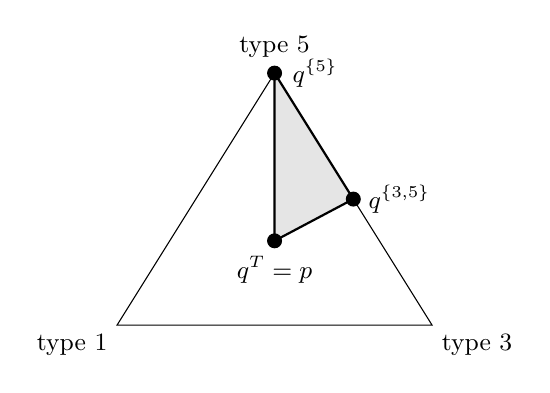
\begin{tikzpicture}[scale=1]
\coordinate (T1) at (0,0);
\coordinate (T3) at (4,0);
\coordinate (T5) at (2,3.2);
\coordinate (W35) at (3,1.6);
\coordinate (Wp) at (2,1.07);
\draw (T1) -- (T3) -- (T5) -- cycle;
\node[below left] at (T1) {\small type $1$};
\node[below right] at (T3) {\small type $3$};
\node[above=2pt] at (T5) {\small type $5$};
\fill[gray!20] (T5) -- (W35) -- (Wp) -- cycle;
\draw[thick] (T5) -- (W35) -- (Wp) -- cycle;
\filldraw (T5) circle (2.5pt);
\filldraw (W35) circle (2.5pt);
\filldraw (Wp) circle (2.5pt);
\node[right=3pt] at (T5) {\small $q^{\{5\}}$};
\node[right=2pt] at (W35) {\small $q^{\{3,5\}}$};
\node[below=2pt] at (Wp) {\small $q^{T}=p$};
\end{tikzpicture}
\caption{The windows at $t=5$ on the running example $T = \{1,3,5\}$, drawn inside the simplex $\Delta(T)$ (one corner per type) at the uniform benchmark. The shaded triangle is the closure of $Q_p(5)$ of Lemma \ref{lem:windows}: its three corners are the window beliefs $q^{\{5\}}$, $q^{\{3,5\}}$, and $q^{T} = p$, nested exactly as the windows $\{5\} \subset \{3,5\} \subset T$ are.}
\label{fig:windows}
\end{figure}

Two boundary rules complete the machinery, stated once and used throughout. First, beliefs in the class are strictly positive, and points added by the closure are never admitted as beliefs: window restrictions other than $q = p$ put zero weight somewhere, so they bound expected payoffs without being available themselves. That is exactly why the lemma's sharp bounds need not be attained inside the class. Second, an entire tied argmax set enters the prediction set from a single belief. Together these decide every knife-edge below: the strict threshold of Example \ref{ex:fpa}(iii), where the binding vertex $q = p$ is the one window restriction inside the class, and the tied-argmax rule by which a ghost bid enters $F_p(t)$ alongside the truthful bid at every belief, in Corollary \ref{th:gaps}.

Everything so far describes the machinery. It now yields a test. Prediction sets consult the payoff rule only where the anchors point, so the mechanism enters through a smaller object than itself.

\begin{definition}[Reduced game]\label{def:reduced}
The \emph{anchored set} is $\beta(T) = \bigcup_{s \in T} B^0(s)$, and the \emph{reduced game} at type $t$ is the array of averaged rows $\bar u(b, \beta(s); t)$ for $b \in A$ and $s \in T$.
\end{definition}

\begin{lemma}[Reduction]\label{lem:reduction}
If two mechanisms on the same $T$ and $A$ induce the same $B^0(\cdot)$ and the same averaged rows, they induce the same $F_p(t)$ at every type and every benchmark.
\end{lemma}

In words: what an agent can be predicted to do depends on the payoff rule only where the rule is consulted. Payoffs against actions no type is conjectured to take never enter the comparison. The anchors themselves are read off the whole menu, so this is a statement about the second stage given the first, not a licence to prune the menu before computing anchors.

\begin{theorem}[Reduced-game dominance]\label{th:dominance}
Fix a type $t$, and for distinct actions $b, b'$ let $\delta^{bb'}$ be the difference vector of Definition \ref{def:diff}.
\begin{enumerate}
\item[i.] Fix a full-support benchmark $p$. Type $t$ is $p$-simple if and only if some $b \in A$ satisfies, for every $b' \neq b$,
\[
\sum_{s \in W} p_s\, \delta^{bb'}_s \;\ge\; 0 \quad \text{for every window } W \text{ at } t,
\]
with strict inequality at $W = T$.
\item[ii.] Type $t$ is robustly simple if and only if some $b \in A$ satisfies, for every $b' \neq b$, $\delta^{bb'} \ge 0$ and $\delta^{bb'} \neq 0$.
\end{enumerate}
\end{theorem}

In words: a type is pinned down at every benchmark exactly when one of its actions beats every alternative against each believed type's anchored play, weakly throughout and strictly against at least one; at a single benchmark the same comparison is weighted, and part (i) gives it. That is dominance, but inside the reduced game rather than the whole mechanism, and it is what gives the measure content: dominant-strategy mechanisms ask for dominance against every action, while robust predictability counts the types with a dominant action against each believed type's anchored play, averaged where an anchor is tied, and predictability at a benchmark counts the types whose weighted comparison in part (i) comes out one way. Proposition \ref{th:sources} is then the anatomy of how the test fails --- a vanishing difference vector is a structural tie, a sign-changing one belief-driven --- and Proposition \ref{prop:attainedtie} says when a failure is behaviourally live.

Part (ii) needs no arithmetic beyond reading signs. Part (i) is what a particular population buys: the same comparison, weighted, and it suffices to check it on the windows at $t$, one sum per consecutive block of types through $t$, with the full block the only one that must come out strictly positive. The test is a conjunction of \emph{pairwise} conditions, so no third action interferes and part (i) needs no argument about which action wins; connectedness enters only in part (ii), and there to rule out the witnessing action changing from one benchmark to another. Each condition is linear in $p$, which fixes the shape of the classification.

\begin{corollary}[Shape of the classification]\label{cor:pwlinear}
Fix $T$, $A$ and the payoff rule. For each type, the set of full-support benchmarks at which it is simple is a finite union of convex cells, each cut out by finitely many linear inequalities, some of them strict. Predictability is piecewise linear on the induced finite partition of the full-support simplex, though it need not be continuous across cell boundaries.
\end{corollary}

The boundaries are hyperplanes, at every $|T|$ and not only at three, because every condition of Theorem \ref{th:dominance}(i) is a linear inequality in $p$. Some of those inequalities are strict --- the full window must come out strictly positive --- so the cells need not be closed and predictability can jump as a boundary is crossed, as it does at the threshold of Example \ref{ex:fpa}. Curvature can enter only through which actions a \emph{sensitive} type is predicted to take, which is a different and harder object; the note closing this section says why.

A prediction can be unique and still be worth almost nothing, and the machinery already assembled measures by how much.

\begin{definition}[Margin]\label{def:margin}
Let $|A| \ge 2$ and let $t$ be $p$-simple with $F_p(t) = \{b\}$. Its \emph{margin} at a belief $q \in Q_p(t)$ is $\min_{b' \neq b} \bigl( U^t_q(b) - U^t_q(b') \bigr)$, and its \emph{floor} at $p$ is the infimum of the margin over $Q_p(t)$.
\end{definition}

\begin{proposition}[Margins]\label{prop:margins}
Let $|A| \ge 2$ and let $t$ be $p$-simple with $F_p(t) = \{b\}$.
\begin{enumerate}
\item[i.] The floor at $p$ is $\displaystyle \min_{b' \neq b} \ \min_{W} \ \frac{1}{p(W)} \sum_{s \in W} p_s\, \delta^{bb'}_s$, the minimum over rivals and over windows at $t$.
\end{enumerate}
Suppose further that $t$ is robustly simple, so that a floor is defined at every full-support benchmark.
\begin{enumerate}
\item[ii.] The floor is zero at every full-support benchmark if and only if $\delta^{bb'}_t = 0$ for some rival $b'$.
\item[iii.] The floor is bounded below by a positive constant not depending on the benchmark if and only if $\delta^{bb'}_s > 0$ for every rival $b'$ and every $s \in T$, and the largest such constant is the least of those values.
\end{enumerate}
\end{proposition}

Part (i) is Lemma \ref{lem:windows} applied to the margin. Against a fixed rival the comparison is affine in the belief, so its infimum over the class is attained at a window restriction --- a point of the closure, not in general a member of the class --- and the margin is the least of these over the finitely many rivals. Part (ii) isolates the worst case, and it has a plain reading: a robustly simple type carries no margin at any benchmark exactly when its predicted action is not the unique best response to the agent's own anchored play, since the singleton window $\{t\}$ is itself a window. Part (iii) is the best case, strict dominance in the reduced game, where the floor survives every benchmark and every belief. Between them sits the ordinary case, a floor positive at each benchmark that shrinks toward zero as the benchmark concentrates on a believed type against which the predicted action holds no strict advantage. The three tiers are what separate the two design instruments of Section \ref{sec:examples}.

Finally, a condition under which the construction reproduces its own input.

\begin{corollary}[Coverage]\label{cor:coverage}
Suppose every $B^0(s)$ is a singleton and every action in $A$ is the anchor of some type. If $t$ is robustly simple with $F_p(t) = \{b\}$, then $B^0(t) = \{b\}$.
\end{corollary}

\begin{corollary}[Ex-post equilibrium]\label{cor:expost}
Suppose every $B^0(s)$ is a singleton and write $\sigma(t)$ for the action predicted at a robustly simple $t$. If every type is robustly simple and $\sigma = \beta$, then $\sigma$ is a weak ex-post equilibrium of the game on $T$, strict against each rival action at some opponent type. Conversely, if $\beta$ is such an equilibrium, then every type is robustly simple.
\end{corollary}

Under coverage, when in addition every type is robustly simple, the conjecture the agents were assumed to form is exactly what the model predicts they do, so iterating the construction returns the same profile and the depth-one commitment costs nothing. That is a fixed point without a common prior, and Corollary \ref{cor:expost} identifies it: predicted play is then a mutual best response under \emph{every} full-support common prior on the perceived grid. Coverage is a hypothesis, not a design principle. It does not deliver predictability by itself --- the first-price example of Section \ref{sec:fpa} has $\beta = (0,1,2)$ covering $A$ and $P(p) = 2/3$ --- and an ex-post equilibrium the reference does not land on says nothing about the measure.

One limitation belongs here rather than in a footnote. Simplicity is a universal over beliefs and therefore factorises into pairs, which is why finitely many window sums settle it. Whether a \emph{given} action belongs to $F_p(t)$ is an existential over beliefs and does not factorise: it is a linear feasibility problem over full-support mixtures of window restrictions. So Theorem \ref{th:dominance} makes predictability exactly computable and leaves the composition of prediction sets at sensitive types where it was.

\section{Applications}\label{sec:examples}

\subsection{A first-price auction: belief-driven sensitivity}\label{sec:fpa}

In a first-price auction, raising one's bid increases the chance of winning but lowers the surplus conditional on winning. Subjective weight on low and high anchored opponents can therefore reverse the preferred bid. The winner pays her own bid, so the payoff is $u(b, b'; t) = (t - b)\bigl[\mathbf{1}(b > b') + \tfrac12 \mathbf{1}(b = b')\bigr]$. Let $T = \{1, 3, 5\}$ and $A = \{0, 1, 2\}$.

\begin{example}\label{ex:fpa}
The reference best responses are unique: $B^0 = (\{0\}, \{1\}, \{2\})$, so the anchor is the pure profile $\beta = (0, 1, 2)$. The classification over full-support benchmarks is:
\begin{enumerate}
\item[i.] Type 1 is robustly simple: $F_p(1) = \{0\}$ for every $p$.
\item[ii.] Type 3 is robustly sensitive: $F_p(3) = \{1, 2\}$ for every $p$.
\item[iii.] Type 5 is $p$-contingent: simple with $F_p(5) = \{2\}$ if and only if $p_3 + \tfrac{3}{2} p_5 > p_1$, with the inequality strict. At equality the undistorted belief $q = p$ attains the tie, so type 5 is sensitive there.
\end{enumerate}
Under the uniform benchmark, predictability is $2/3$ and revenue over selections from the prediction sets lies in $[13/9,\, 16/9]$. 
%All statements verified in exact arithmetic.
\end{example}

The driving identities are short. For type 3, the payoff rows of bids 1 and 2 against $\beta$ are $(2, 1, 0)$ and $(1, 1, \tfrac12)$, so $U^3_q(1) - U^3_q(2) = q_1 - \tfrac12 q_5$; types 1 and 5 lie on opposite sides of 3, and centredness constrains each side separately, placing no restriction on their relative weight, so both signs are attained at strictly positive beliefs for every $p$, while $U^3_q(1) - U^3_q(0) = \tfrac12 q_1 + q_3 > 0$ keeps the pair $\{1,2\}$ on top. For type 5 the same computation gives $U^5_q(2) - U^5_q(1) = -q_1 + q_3 + \tfrac32 q_5$; whether some centred belief makes this nonpositive is decided at the window restrictions (Lemma \ref{lem:windows}): up to positive scale, the three windows at type 5 evaluate it to $\tfrac32 p_5$, $p_3 + \tfrac32 p_5$, and $-p_1 + p_3 + \tfrac32 p_5$, all positive exactly when $p_3 + \tfrac32 p_5 > p_1$, the threshold in (iii). The remaining comparison, $U^5_q(1) - U^5_q(0) = \tfrac32 q_1 + 2 q_3 > 0$, removes bid 0 and completes the classification. Under the uniform benchmark the anchor coincides with a Bayes--Nash equilibrium of the true game; this coincidence is example-specific and fails for $T = \{2, 3, 6\}$.

Type 3 illustrates the reading of sensitivity given above. Its two neighbours sit on opposite sides, and the class allows their relative weight to be tilted either way; no symmetry requirements are posted, so the analyst's stance does not determine which bid it submits. An analyst prepared to assume that distortion depends on distance $|t-s|$ alone would call type 3 simple under the uniform benchmark $p$, since $U^3_q(1) - U^3_q(2)$ would then be proportional to $p_1 - \tfrac12 p_5$ and always positive. Type 1 is simple at every benchmark under the wide class, so no strengthening can make it sensitive; type 5 likewise stays simple wherever the threshold above puts it in the simple region.

Grid design is already visible. Remove bid 2: on $A = \{0, 1\}$ the anchors are $(0, 1, 1)$, and every type's best response is belief-free: $F_p(1) = \{0\}$, $F_p(3) = \{1\}$, $F_p(5) = \{1\}$, with every pairwise payoff difference strictly signed at every centred belief. So predictability is $1$ at every benchmark, against $2/3$ at the uniform benchmark on $\{0, 1, 2\}$. The gain is bought by capping bids at 1.

The cap is worth stating in general, because with two bids the whole construction collapses to one comparison and the answer can be read off the grid.

\begin{corollary}[Two-bid caps]\label{prop:cap}
Let the payoff rule be first-price, let $A = \{a_1, a_2\}$ with $a_1 < a_2$, and write $\theta = \tfrac{1}{2}(3 a_2 - a_1)$.
\begin{enumerate}
\item[i.] $B^0(t) = \{a_2\}$ for $t > \theta$, $B^0(t) = \{a_1\}$ for $t < \theta$, and $B^0(\theta) = \{a_1, a_2\}$.
\item[ii.] For a type $t$, the difference vector of $a_2$ over $a_1$ is
\[
\delta_s \;=\;
\begin{cases}
\tfrac12\,(t + a_1 - 2a_2), & s < \theta, \\[2pt]
\tfrac12\,(t - \theta),     & s = \theta, \\[2pt]
\tfrac12\,(t - a_2),        & s > \theta,
\end{cases}
\]
and these three values increase in that order.
\item[iii.] Type $t$ is robustly simple if and only if the values $\delta_s$ taken on $T$ are of one weak sign and not all zero.
\end{enumerate}
\end{corollary}

In words: a two-bid menu sorts the opponents the agent might face into those the reference sends to the high bid, those it sends to the low one, and at most one at the cutoff itself, whose conjectured play is the even mixture of the two, and the agent's own comparison is then a single advantage number per believed opponent, larger against opponents believed to bid high. The agent's bid is pinned down whatever it believes exactly when that number never changes sign across the opponents it might face and is not zero against every one of them. When it does change sign, some composition of the opponent population balances the two bids exactly, and at such a benchmark the agent's perception can attain the tie.

By Definition \ref{def:predictability}, $P(p) = 1$ at every full-support benchmark exactly when every type is robustly simple, so part (iii) settles the cap. The condition it gives is an interval condition on the grid.

\begin{corollary}[Dead zone]\label{cor:deadzone}
Let the payoff rule be first-price with $A = \{a_1, a_2\}$, $a_1 < a_2$, and write $D(A) = \bigl(a_2,\; 2a_2 - a_1\bigr)$. If $T$ contains types strictly on both sides of $\theta$, then $P(p) = 1$ at every full-support benchmark if and only if $T \cap D(A) = \emptyset$.
\end{corollary}

The dead zone is an open interval of length $a_2 - a_1$ lying immediately above the cap. Under the corollary's hypothesis --- values on both sides of the cutoff, and predictability demanded at every benchmark --- a cap works exactly when no perceived value falls just above it. Off that hypothesis the operative interval is narrower, as the next paragraph explains. A value below the cap is served by the low bid and a value well above it by the high bid, but a value in between is served by whichever bid the agent's perception favours.

The scope clause is load-bearing, and a tied reference is where it bites. The three values of part (ii) vanish at the three points $a_2 < \theta < 2a_2 - a_1$, and the operative dead zone is the open interval between the zeros of the smallest and the largest value actually realised on $T$ when those differ, and the single point where they coincide otherwise (see the proof in Appendix \ref{app:proofs}). They coincide when $T$ lies strictly on one side of $\theta$, and also when $T = \{\theta\}$, where the realised vector is identically zero and the type is sensitive. Types strictly on both sides of $\theta$ realise both outer values, and the interval is $D(A)$ itself. Otherwise it shrinks: a type set that reaches $\theta$ from below without passing it has dead zone $(\theta,\, 2a_2 - a_1)$, one that reaches it from above has $(a_2,\, \theta)$, and a type set staying strictly on one side has a dead zone that collapses to the single point where its one realised value vanishes. This is why $A = \{2,4\}$ against $T = \{1,3,5\}$, whose reference ties at type 5, is robustly simple all the same.

A working cap does one of two things, and which one is settled before any belief is named.

\begin{corollary}[Separate or pool]\label{cor:sepool}
Let the payoff rule be first-price and let every type be robustly simple on $A = \{a_1, a_2\}$. If $T$ lies weakly on one side of $\theta$, every type takes the same bid: $a_1$ if $T$ lies below, $a_2$ if above. Otherwise every $t < \theta$ takes $a_1$ and every $t > \theta$ takes $a_2$.
\end{corollary}

Either the possible values lie on one side of the cutoff, so no agent's advantage number can change sign and the whole population pools; or they straddle it, and the cap sorts the types cleanly on either side. Nothing between survives, because a type inside the operative dead zone faces advantage numbers of both signs. A cap can also be chosen from a lower bound on the values alone, knowing nothing else about the grid --- the opposite of what alignment will demand below --- and one way is to set the cap far enough below every value --- the headroom between the cap and the lowest value at least the spread between the two bids, which is Corollary \ref{cor:floor}'s hypothesis --- so that every type bids it and predictability comes by pooling rather than by separation (Corollary \ref{cor:floor}, in the appendix). A lower bound on values therefore guarantees full predictability, at the price of collapsing the prediction to a single bid; the guarantee question with content is the one that also asks for separation, or for revenue, or for a margin, and we do not take it up here. That inequality is demanding: no two-bid grid on $\{0,\dots,5\}$ satisfies $2a_2 - a_1 \le \min T$ against $T = \{1,3,5\}$.

Predictability is one thing and the strength of a prediction another. Proposition \ref{prop:margins} separates them here.

\begin{corollary}[First-price margins]\label{cor:fpmargins}
Let the payoff rule be first-price, let $|A| \ge 2$, and let $t$ be robustly simple.
\begin{enumerate}
\item[i.] If $B^0(t) = \{a^*\}$ is a singleton, the floor of $t$ is zero at every benchmark if and only if the bid $(t + a^*)/2$ lies in $A$ above $a^*$ and the predicted bid is $a^*$ or that bid.
\item[ii.] On a two-bid menu no such configuration exists, and the floor is zero at every benchmark exactly at a type whose reference ties, that is at $t = \theta$.
\end{enumerate}
\end{corollary}

Against an opponent at the anchor $a^*$ a bid earns nothing if it loses, $\tfrac12(t - a^*)$ if it ties, and $t - b$ if it wins; the tie and a win at $b$ are worth the same exactly when $b = (t + a^*)/2$. That coincidence needs a third bid to exist, so Corollary \ref{prop:cap} cannot see it, and the scope matters: with three or more bids a cap can pin every type down and still leave some prediction defended by nothing. On two bids the only such types sit at the cutoff, where the reference is tied rather than singleton and the two bids average to $\tfrac14 (t - a_1)$ and $\tfrac34 (t - a_2)$, equal precisely at $\theta$ --- so part (ii) is a statement about tied anchors, and Section \ref{sec:ties} is where such types are studied. A tied anchor at $\theta$ does not make a type sensitive: on $A = \{2,4\}$ against $T = \{1,3,5\}$ the reference ties at type 5, which is robustly simple all the same, and it is precisely there that its prediction is defended by nothing.

Predictability, separation and a margin that survives every benchmark can hold together, though the running grid is too coarse to show it.

\begin{example}\label{ex:strict}
Take $T = \{\tfrac12, 3, 5\}$ and $A = \{0, 1\}$, so $\theta = \tfrac32$ and the closed interval $[a_2, 2a_2 - a_1] = [1,2]$ contains no value. The anchors are $B^0 = (\{0\}, \{1\}, \{1\})$. Type $\tfrac12$ bids $0$ and types $3$ and $5$ bid $1$, so the cap separates; the difference vectors of the predicted bid over its rival are $(\tfrac34, \tfrac14, \tfrac14)$, $(\tfrac12, 1, 1)$ and $(\tfrac32, 2, 2)$, all strictly positive, so by Proposition \ref{prop:margins}(iii) the margins are at least $\tfrac14$, $\tfrac12$ and $\tfrac32$ at every belief and every benchmark.
\end{example}

Every action here is the anchor of some type, so Corollary \ref{cor:coverage} applies: the predicted profile is the anchor profile, and by Corollary \ref{cor:expost} it is a weak ex-post equilibrium on the perceived grid. A two-bid first-price menu whose dead zone is clear of values therefore has a pure ex-post equilibrium, and the construction finds it from the uniform reference alone. Against $T = \{1,3,5\}$ on $\{0,\dots,5\}$ no straddling cap clears the closed interval, which is why the running example cannot display this.


Belief-driven sensitivity is thus a grid phenomenon, and the grid a design instrument. That the action menu is something a designer actually sets is not hypothetical: exchanges fix the minimum price increment, and regulators have changed it deliberately, as in the 2016--18 tick size pilot. We cite that only as an instance of the lever being pulled. Its measured effects concern spreads and depth in a dynamic, many-sided market with an interdependent-value component, all of which lie outside the present model. The second-price auction next shows sensitivity of a different origin.
%, which no grid touches.

\subsection{A second-price auction: structural sensitivity}\label{sec:spa}
% In the following example, the best responses to uniform reference seem unique at truthful bidding for each type, as the 'uniqueness here is a theorem' stated. Yet, the structurally sensitive depends not only on payoff rule, but also the gap in type perceptions: no type 2 yet action 2 exists, it may partially explain why ideal predictions in smooth setting cannot be experimentally examined, yet referees would challenge this as ad hoc, not a meaningful contribution.
In a second-price auction, one's bid changes the allocation but not the payment conditional on winning. Truthful bidding therefore anchors every type when the truthful bid is available. Yet gaps between anchored values can leave several bids payoff-equivalent at the prediction stage. The winner pays the opponent's bid, so the payoff is $u(b, b'; t) = (t - b')\mathbf{1}(b > b') + \tfrac12 (t - b)\mathbf{1}(b = b')$. Keep $T = \{1,3,5\}$ and let $A = \{0, 1, \dots, 5\}$.

The next lemma makes the first-stage anchor claim precise.

\begin{lemma}[Truthful anchor]\label{lem:truthful}
Let the payoff rule be second-price. If $T \subseteq A$, then $B^0(t) = \{t\}$ for every type under the uniform reference. Indeed, this holds under any full-support reference.
\end{lemma}

So the anchor is truthful, the mixture of Definition \ref{def:anchor} degenerate, and an apparent paradox dissolves: a strictly unique anchor is followed by total sensitivity. At the anchor stage, beliefs cover every bid in $A$: for type 3, bids 2 and 4 carry positive weight, and bid 3 strictly beats both. At the prediction stage, opponents play only the anchored bids $\beta(T) = \{1, 3, 5\}$, and against these, bids 2, 3, and 4 all earn the payoff row $(2, 0, 0)$. Uniquely separated at the reference, payoff-equivalent against anchored play: structural sensitivity lives in the \emph{reduced game} --- play against anchored bids only --- generated by $\beta(T)$, not in $A$ itself.

\begin{example}\label{ex:spa}
Every type is structurally sensitive, for every full-support benchmark and every centred belief:
\[
F_p(1) = \{0, 1, 2\}, \qquad F_p(3) = \{2, 3, 4\}, \qquad F_p(5) = \{4, 5\},
\]
and within each set the expected-utility differences are identically zero. Predictability is $0$ at every benchmark. Under the uniform benchmark, with the two values drawn independently from it, revenue over selections lies in $[10/9,\, 3]$, with the truthful revenue $19/9$ strictly inside. The classification above is benchmark-free; these revenue figures are not. 
\end{example}

One ghost bid, worked in full, shows the mechanism. Take type 3 and compare its truthful bid with the unanchored bid 4, event by event against the three anchored bids:
\[
\begin{array}{lccc}
& \text{opponent bids } 1 & \text{opponent bids } 3 & \text{opponent bids } 5 \\[2pt]
\text{bid } 3: & 3 - 1 = 2 & \tfrac12(3 - 3) = 0 & 0 \\[2pt]
\text{bid } 4: & 3 - 1 = 2 & 3 - 3 = 0 & 0
\end{array}
\]
The payoff rows agree everywhere. The two bids disagree only about the allocation against the middle opponent (bid 3 ties it, bid 4 beats it outright), and that is exactly the opponent whose bid equals the bidder's own value, so winning there is worth nothing either way. A bid strictly inside a gap changes the allocation only at price-equals-value events, where the payoff is unaffected either way. This is also why the second-price classification is benchmark-free while the first-price threshold of Example \ref{ex:fpa}(iii) moves with $p$: identical rows tie at every belief and every benchmark, whereas a nonzero difference merely balances at some.

The structural ties sit exactly in the gaps between values, and the geometry is complete.

\begin{corollary}[Gaps]\label{th:gaps}
Let the payoff rule be second-price and let $T \subseteq A$. The \emph{adjacent gaps} of a type $t$ are the two open intervals separating it from its neighbouring values, and, when $t$ is the lowest or the highest value, the unbounded interval on that side --- below $\min T$, or above $\max T$. For each type $t$ the following are equivalent:
\begin{enumerate}
\item[i.] $t$ is $p$-sensitive at some full-support benchmark;
\item[ii.] $t$ is $p$-sensitive at every full-support benchmark;
\item[iii.] some bid in $A$ lies strictly inside an adjacent gap of $t$.
\end{enumerate}
Consequently predictability is the benchmark mass of the types with no bid in either adjacent gap.
\end{corollary}

In words: a bid strictly inside one of a type's own adjacent gaps is a ghost for that type --- no anchored opponent is conjectured to bid there --- so it earns exactly what the truthful bid earns against every anchored opponent. The allocations differ against the one opponent bidding the agent's own value, where truth ties and the ghost does not, but there winning is worth nothing, so the payoffs agree and nothing in the prediction can tell the two apart. A type is unpredictable precisely when the grid offers it a ghost bid on one side or the other. In the proof, weak dominance does double duty: it hands every structural tie with the truthful bid its attainment for free.

\begin{figure}[H]
\centering
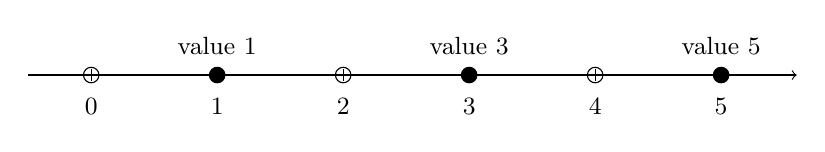
\begin{tikzpicture}[x=1.6cm]
\draw[->] (-0.5,0) -- (5.6,0);
\foreach \x in {0,...,5} \draw (\x,0.08) -- (\x,-0.08);
\foreach \x in {1,3,5} { \filldraw (\x,0) circle (2.8pt); \node[above=4pt] at (\x,0) {\small value $\x$}; }
\foreach \x in {0,2,4} \draw (\x,0) circle (2.8pt);
\foreach \x in {0,...,5} \node[below=5pt] at (\x,0) {\small $\x$};
\end{tikzpicture}
\caption{The gap geometry of Corollary \ref{th:gaps} on the running example. Filled bids sit at the perceived values; open bids are ghosts, each strictly inside some value's adjacent gap. On $A = \{0, \dots, 5\}$ every value has an adjacent ghost, so predictability is zero. Deleting the ghosts (alignment, $A = T$) makes every type simple, at the price of knowing the latent grid $T$; the margins are thin under every second-price grid that keeps each value biddable, aligned or not (Corollary \ref{cor:spamargins}).}
\label{fig:gaps}
\end{figure}

\begin{corollary}[Alignment]\label{cor:align}
In the second-price auction with $T\subseteq A$, Corollary \ref{th:gaps} gives $P(p)=1$ at some (equivalently every) full-support benchmark iff $A=T$. Under alignment, every type satisfies $F_p(t)=\{t\}$ at every full-support benchmark.
\end{corollary}

Both directions lean on $T \subseteq A$, and the dependence is not cosmetic: the truthful-anchor lemma and the gap geometry each require the true values to be feasible bids. Alignment also removes every structural tie, so it delivers predictability. What it does not deliver is a prediction worth much, and the reason is the payment rule rather than the instrument.

\begin{corollary}[Second-price margins]\label{cor:spamargins}
Let the payoff rule be second-price with $T \subseteq A$ and $|A| \ge 2$. For every type and every rival bid the difference vector vanishes at the agent's own type. Hence by Proposition \ref{prop:margins}(ii) the floor of every robustly simple type is zero at every full-support benchmark, on every grid keeping each value biddable, aligned or not. By Corollary \ref{th:gaps} a simple type here is robustly simple, so the restriction costs nothing.
\end{corollary}

The reason is one line: against an opponent bidding the agent's own value, winning means paying exactly that value, so every bid earns nothing and no bid can be preferred. Under alignment the margin against an underbid $b$ is at least $q_b \cdot \tfrac12 (t - b)$, positive at every centred belief, so the prediction really is unique; but it shrinks to zero as perception concentrates on the own type, and this is not a cost of alignment. It is a feature of paying the loser's bid, and among grids that keep every value biddable no choice removes it. Off that scope the conclusion can fail: on $T = \{1,3\}$ with $A = \{0,2\}$, type 3 has advantage vector $(1, \tfrac12)$ and so a floor of $\tfrac12$ at every benchmark. The contrast with the cap is the point: any small thing the model leaves out --- a rounding of the payments, a slight cost of thinking the comparison through --- could flip a second-price prediction, and by Corollary \ref{cor:fpmargins} a first-price cap on two bids leaves no such opening except at the cutoff itself, for a type pinned down at every benchmark. The floor concerns the anchored payoff rows as they stand, so what it protects against is a perturbation on the agent's side, not a change to the mechanism, which would move the anchors as well.
 
The cap behaves differently, and the contrast is what makes the point worth making. On $A = \{0,1\}$ Corollary \ref{prop:cap}(ii) gives the margins directly. The bidder worth 3 prefers bid 1 to bid 0 by $1 - \tfrac12 q_1$, and the bidder worth 5 by $2 - \tfrac12 q_1$; since $q_1$ is a probability and so at most one, these never fall below $\tfrac12$ and $\tfrac32$ respectively, whatever the two believe. The bidder worth 1 is the different case. Her margin is $\tfrac12 q_1$, proportional to the weight she places on bidders like herself and with no constant term to hold it up, so what it needs is a floor under $q_1$ rather than a ceiling over it. Centredness supplies one --- her own type is the one she overweights most relative to the benchmark, and those overweightings average to one, so she cannot underweight it --- giving $q_1 \ge p_1$ and a margin of at least $\tfrac12 p_1$. Every margin is therefore bounded away from zero before any belief is named: two of them by the payoff rule alone, the third by the benchmark. In the terms of Proposition \ref{prop:margins}, the bidders worth 3 and 5 sit in tier (iii) and the bidder worth 1 in the ordinary middle case, her floor positive at each benchmark but shrinking with $p_1$. The second-price rule offers no floor at all, on any grid keeping every value biddable.

One thing alignment does deliver, and it is not about margins. Every value is then the anchor of some type and every bid is a value, so Corollary \ref{cor:coverage} applies: the predicted profile is the anchor profile, truthful bidding, and by Corollary \ref{cor:expost} it is a weak ex-post equilibrium on the perceived grid. Both design instruments therefore share this property --- the aligned second-price menu and the working two-bid cap of Example \ref{ex:strict} alike --- and they share it for the same reason, that every action they leave available is one some type is conjectured to take. It is a consequence the two repairs happen to have in common, not a principle either was built on, and mechanisms in general do not have it.

Without $T \subseteq A$ the equivalence fails: grids missing the values can also reach full predictability, even a two-bid grid missing both values, with the low type's anchor tied ($T = \{1,3\}$, $A = \{0,2\}$), so the repair claim is scoped to grids that keep truthful bidding available.

Alignment is the second design instrument, and its cost is a demand for information. The instrument requires the designer to match the perceived value grid $T$ exactly, a primitive of the model here, whose recovery from observed bidding is a separate identification problem the framework poses but this paper does not solve. A cap need not make that exact match, but it does need to keep its operative dead zone clear. Corollary \ref{cor:deadzone} locates the knife-edge for the case that matters: when the possible values fall on both sides of the reference cutoff, a two-bid menu delivers full predictability at every benchmark exactly when no value lies strictly inside the interval of length $a_2 - a_1$ immediately above the cap. Against $T = \{1,3,5\}$, Corollary \ref{prop:cap} settles all fifteen two-bid grids on $\{0,\dots,5\}$. Thirteen make every type robustly simple; the two that fail are $\{0,2\}$, whose dead zone $(2,4)$ catches the value 3, and $\{0,3\}$, whose dead zone $(3,6)$ catches the value 5. Both failures sit at the prediction stage: $\{0,2\}$ also ties its reference, but that tie is not what breaks it, since resolving $B^0(3)$ to either bid still leaves type 3 sensitive at some benchmark. The corollary's scope is what saves three of the other thirteen. On $\{0,4\}$, $\{1,4\}$ and $\{2,4\}$ a value does sit above the cap by less than the spread, but no value lies above the reference cutoff, so the cap is never in contention and every type takes the low bid whatever it believes --- $\{2,4\}$ ties its reference at type 5 into the bargain, and is robustly simple regardless. What a cap needs is therefore a property of the cap and the value grid together. It is weaker than what alignment demands, but it is not nothing.

\section{Tied anchors}\label{sec:ties}

The numbered examples above use unique anchors. The first-price menu below deliberately creates a tie. When a reference best-response set is tied, Axiom \ref{ax:neu}(ii) makes the conjecturer spread weight uniformly across it. This remains a statement about unresolved conjecture, not observed mixed behaviour. We compute the resulting prediction here; the check against alternative scenarios that resolve each tie purely is carried out in Appendix \ref{app:resolutions}.



Return to the first-price rule and remove the middle bid: $T = \{1, 3, 5\}$, $A = \{0, 2\}$. Against the uniform reference, type 1 strictly prefers 0 and type 5 strictly prefers 2, but type 3 is exactly indifferent: $B^0(3) = \{0, 2\}$. Here the anchor of type 3 is the uniform mixture on $\{0, 2\}$, and the theory runs unchanged.

\begin{example}\label{ex:tied}
The averaged payoff rows of type 3's two bids against the anchor profile are $\bar u(0, \beta(\cdot); 3) = (\tfrac32, \tfrac34, 0)$ and $\bar u(2, \beta(\cdot); 3) = (1, \tfrac34, \tfrac12)$, so
\[
U^3_q(0) - U^3_q(2) \;=\; \tfrac12 q_1 - \tfrac12 q_5 ,
\]
and both signs are attained at strictly positive centred beliefs for every benchmark: type 3 is robustly sensitive with $F_p(3) = \{0, 2\}$. Types 1 and 5 are robustly simple, $F_p(1) = \{0\}$ and $F_p(5) = \{2\}$, so predictability is $P(p) = p_1 + p_5$ at every benchmark. 
\end{example}

The instance teaches two distinctions cleanly. First, type 3's two bids tie \emph{at the reference}, but they are not payoff-equivalent against anchored play: their rows differ, and $U^3_q(0) - U^3_q(2)$ moves with the belief. The sensitivity is therefore belief-driven, not structural: a reference tie concerns the anchor stage, a structural tie concerns the prediction stage, and neither implies the other. Second, robustness itself is not a structural signature: type 3's tie is attained at every benchmark only because the two opponent types driving it, 1 and 5, sit on opposite sides with no constraint linking their relative weight, so both signs of $U^3_q(0) - U^3_q(2)$ stay reachable whatever $p$ is, a belief-driven route to the same robustness that Section \ref{sec:spa}'s structural ties reach by weak dominance instead (Remark \ref{rem:originreach} develops the contrast). The second-price auction makes the same point from the opposite side: a strictly unique reference best response followed by structural ties against anchored play.

The instance also passes a check on Axiom \ref{ax:neu}(ii): at the uniform benchmark, resolving the tie to either pure conjecture collapses type 3's prediction to a singleton that depends on the arbitrary choice, while the equal-weight conjecture reports the union $\{0,2\}$ and the predictions of types 1 and 5 are unmoved. On a two-action menu the union always contains the equal-weight prediction.

\begin{corollary}[Two actions]\label{cor:binary}
If $|A| = 2$, then $F_p(t) \subseteq \bigcup_{\gamma} F^{\gamma}_p(t)$ for every type and benchmark, where $\gamma$ ranges over the pure resolutions of the tied sets.
\end{corollary}

Beyond two actions the containment can fail in both directions, and the machinery behind the check --- resolutions, the pairwise identity, a worked failure, and the finer anatomy of structural ties --- is collected in Appendix \ref{app:resolutions}.

Finally, the two faces of a tied anchor. Both are first-price menus on $T = \{1,3,5\}$ whose reference ties at $\theta$, and they behave oppositely: here $T = \{1,3,5\}$ straddles the cutoff $\theta = 3$ of the menu $A = \{0,2\}$, the realised advantage numbers change sign, and the tied type is robustly sensitive; whereas $A = \{2,4\}$ leaves $T$ weakly on one side of $\theta = 5$, so the tied type 5 is robustly simple and yet, by Corollary \ref{cor:fpmargins}(ii), its prediction is defended by nothing. The same tie, both outcomes, and which one occurs is settled by where $T$ sits relative to the cutoff.

\section{Related literature}\label{sec:literature}

The paper's family is the subjective-belief tradition: projection \citep{gpr2021projection}, cursed beliefs \citep{eyster2005cursed}, analogy-based expectations \citep{jehiel2005analogy}, and level-$k$ reasoning \citep{crawford2007levelk} all replace correct forecasts with structured misperception. Any such model whose conjecture is a centred reweighting of the benchmark applied to anchored play, and which maximises the expected payoff of Definition \ref{def:payoff}, selects a point inside our prediction sets by construction, and the framework is the envelope over those variants, identifying where the selection matters. Projection toward the agent's own type and the level-$k$ second step at $q = p$ both qualify; cursed and analogy-based expectations are kin rather than instances, their conjectures not being of that form. The method is robust mechanism design transplanted to the agents' side: a class of beliefs replaces a point belief, and conclusions are reported over the whole class. The simplicity literature is the neighbour we measure rather than join: obviously strategy-proof mechanisms \citep{li2017osp} and strategically simple mechanisms \citep{borgersli2019strategically} are classes (a mechanism is in or out) certifying that the agent can find its optimal strategy, while predictability is a measure, defined for every mechanism of the finite static kind studied here, of whether the analyst can call the play. The two axes cross in the sealed-bid second-price auction: strategy-proof, strategically simple, and (on the running grid, where every value has a bid in an adjacent gap) predictability zero; under that rule with every value biddable, sensitivity falls exactly on the types whose adjacent gaps hold a bid (Corollary \ref{th:gaps}). The newest instance of the same axis is \citet{zhang2026gda}, who buys belief-freeness by restricting to dominant-strategy mechanisms and then optimises a worst-case guarantee over the value distributions consistent with one coarse statistic. That is joining the class in order to optimise; predictability instead asks, of any mechanism, how much of behaviour survives the removal of the agents' distributional knowledge --- a quantity that is zero at a dominant-strategy mechanism on the running grid, and one at a first-price cap: on $A = \{0,1,2\}$ against $T = \{1,3,5\}$ type 3 has no dominant bid, while on $A = \{0,1\}$ every type does (Corollary \ref{cor:coverage}). One honesty note carries through: the second-price results are reference-free where every value is biddable, holding for every full-support reference, while first-price classifications are relative to the anchor, and we report them as such.

The finite primitives also have their own literature. Evidence indicates that people do not carry continuous distributions into decisions: probability assessment is cognitively costly and distorted under complexity \citep{enke2023cognitive}, reasoning proceeds through a finite number of categories \citep{mss2008coarse}, opponents' contingencies are bundled into coarse classes \citep{jehiel2005analogy}, costly attention makes choice coarse and stochastic \citep{matejka2015rational}, and information-constrained decisions concentrate on finitely many actions even in continuous environments \citep{jung2019discrete}. Discreteness also matches how equilibrium analysis is actually done: closed-form auction equilibria exist only under strong assumptions, and beyond them equilibria are computed on discrete grids \citep{bichler2025computing}, a passage that can change strategic structure qualitatively \citep{rasooly2020discrete}. The equilibrium benchmark is also computationally out of reach in the worst case: with discrete values and bids, even deciding whether a pure-strategy equilibrium exists is NP-hard, and approximate equilibria are as hard as general fixed-point computation \citep{filosratsikas2023complexity}. Our finite primitives carry no such special structure (any finite grids, any private-values payoff, any benchmark), and their prediction questions become finite linear-feasibility problems over mixtures of the window restrictions in Lemma \ref{lem:windows}. The finite model is therefore the general object, not a solvable special case. The finite type space here is a model of the agent's coarse view of its opponents, not of the physical environment. This coarseness is not decorative: gaps between perceived values are what structural sensitivity and its design geometry live on in the second-price auction, and they exist only because perception is coarse.

\section{Concluding remarks}\label{sec:outlook}

This draft delivers the foundation: one axiom, an anchored depth-one construction, centred perceptions, and predictability as the measure; the two origins of sensitivity separated by the auctions, the grid a design instrument against both origins (caps for belief-driven sensitivity, characterised here for two-bid menus, when the values straddle the reference cutoff, by a dead zone just above the cap, exact alignment for structural, the latter knife-edge), and the axiom's second clause checked against pure resolutions. Two of those pieces are now theorems. The origin split rests on a dichotomy on payoff rows, since prediction sets depend on the mechanism only through the anchors and the anchored columns (Lemma \ref{lem:reduction}) and robust simplicity is dominance in the game those columns define, with simplicity at a given benchmark its weighted form (Theorem \ref{th:dominance}); the classification regions are consequently cut by hyperplanes at every number of types, not by curves (Corollary \ref{cor:pwlinear}). What remains open is the companion question: whether a given action is \emph{ever} predicted is a linear-feasibility problem over mixtures of window restrictions whose resulting belief has full support, and unlike simplicity it does not reduce to pairwise comparisons. Design then becomes a trade-off frontier, predictability against revenue, moved by grids, by payment perturbations that delete structural ties, and by menus. Predictability does not move in one direction under menu inclusion, because a bid enters twice, first in the uniform reference and then in the prediction stage: deleting even a never-anchored bid can overturn another type's prediction, and it can move predictability in either direction.\footnote{For an exact first-price witness at the uniform benchmark, take $T=\{1,6\}$ and $A=\{0,3,4\}$. The anchors are $(0,4)$ and type 6 has $F_p(6)=\{0,3,4\}$, although bid 3 is never anchored. Deleting bid 3 changes the anchors to $(0,\{0,4\})$ and leaves $F_p(6)=\{0\}$. In the other direction, take $T=\{2,4,6\}$ and $A=\{0,1,3\}$. The anchors are $(1,3,3)$, so bid 0 is anchored by no type; every type is simple and $P(p)=1$. Deleting bid 0 leaves the anchors unchanged but makes type 4 sensitive, and $P(p)=\tfrac23$.} Grid choice is therefore optimisation rather than refinement in one direction. Two closures deserve naming, and they are different objects. An agent might impose its own subjective belief on the opponent and solve the resulting misspecified equilibrium: coherent, but demanding a fixed point from agents whose limitation is the model's premise. Or the construction itself might be iterated, each agent best responding to the predictions the model assigns its opponents rather than to their anchors alone. The second is internal to the framework, and it is the one the depth-one commitment leaves open. Neither closure delivers a Bayes--Nash equilibrium in general, and not for want of effort: absent a common prior there is no single distribution against which a Bayes--Nash mutual best response would be defined, so recovering that fixed point would mean supplying the common prior the framework sets out to do without.
 
Of the iterated construction one thing can be said already. Under the second-price rule, where every value is biddable, bidding one's value weakly dominates and so is a best response against every conjecture at every depth; it therefore lies in every prediction set the iteration produces, and in any fixed point the iteration may have. More can be said at two instruments in particular: alignment, where the anchors are the values and the values are the bids, and the cap of Example \ref{ex:strict}, whose two bids are anchored by types $\tfrac12$ and $3$. At those two every available action is the anchor of some type and every type is robustly simple, so by Corollary \ref{cor:coverage} the predicted profile is the anchor profile: the construction is stationary there, every further round returns the same profile, and the depth-one commitment costs nothing. By Corollary \ref{cor:expost} that profile is a weak ex-post equilibrium on the perceived grid, so the sentence above needs its scope --- no closure delivers a Bayes--Nash equilibrium in general, but at those two the construction reaches something stronger than one, a profile robust to every full-support common prior. Being a working cap is not enough: the cap $\{2,4\}$ against $T = \{1,3,5\}$ pins every type down, but type 5's anchor is the tied mixture and no type anchors bid 4 alone, so Corollary \ref{cor:coverage} does not apply to it. Stationarity at two points says nothing about uniqueness or about convergence from elsewhere. What cannot yet be said is whether the iteration converges in general, whether a fixed point is unique, or what survives beside value-bidding. The first step widens rather than narrows --- from anchors at the values it returns the wider sets of Example \ref{ex:spa} --- so we do not assert convergence, and we leave the iterated construction, with the selection question it raises, to future work.

The framework also converts an empirical question into a precise one. Under the second-price rule with every value biddable, the gap geometry says that each bid the model admits for a type, other than that type's own value, lies strictly inside one of its adjacent gaps. That makes the perceived grid a recoverable object, at least in principle.

\begin{remark}[Recovery]\label{rem:recovery}
Let the payoff rule be second-price with $T \subseteq A$ and $|T| \ge 2$. The family $\{F_p(t)\}_{t \in T}$ determines $T$, and no benchmark enters: for each type, its predecessor in $T$ is the largest bid in $A$ below the least element of its prediction set, and its successor the smallest bid above the greatest, whenever these exist.
\end{remark}

That is a statement about the model, not about data: Corollary \ref{th:gaps} gives $F_p(t) = A \cap (t^-, t^+)$, so the map from a perceived grid to its family of prediction sets is injective and can be inverted by reading off the two bids just outside each set. Nothing about the benchmark is used, because nothing about the benchmark enters those sets.

Turning that into an empirical procedure is a programme rather than a result, and its content is what the remark does not supply: an observation model, linking what is seen to the whole prediction set rather than to one draw from it; data in which a type's bid support is observable at all; and above all a treatment of the agent's own value, since the prediction set is indexed by a perceived type and recovering the grid presumes the agent reasons with a cell rather than a point. That last is the limitation already noted above, and it is the one that decides whether the exercise is possible.

Both quantities the paper defines are computable from the mechanism and the perceived grid before any behaviour is observed. Without the benchmark one can still compute which types are robustly simple, and for each of those the benchmark-free bound of Proposition \ref{prop:margins}(iii); neither is predictability itself nor the floor at a given benchmark, both of which need $p$.

\appendix

\section{Proofs}\label{app:proofs}

\begin{proof}[Proof of Proposition \ref{prop:reference}]
Fix two actions $b, b' \in A$ and let $\pi$ be the permutation that exchanges $b$ and $b'$ and fixes every other action. Invariance to renaming requires $R_A(\pi(b)) = R_A(b)$, that is, $R_A(b') = R_A(b)$: exchanging any two actions must leave their weights unchanged, so those two weights are equal. Since $b, b'$ were an arbitrary pair, every action carries the same weight, say $c$. As $R_A \in \Delta(A)$, the weights sum to one: $|A| \cdot c = 1$, so $c = 1/|A|$, and $R_A$ is the uniform distribution. Conversely, the uniform distribution assigns $1/|A|$ to every action; any permutation only relabels which action receives which weight, and every weight equals $1/|A|$, so the distribution is unchanged. The uniform distribution is therefore the unique element of $\Delta(A)$ invariant under every permutation.
\end{proof}

\begin{proof}[Proof of Remark \ref{rem:mono}]
Since $Q'_p(t) \subseteq Q_p(t)$, the union defining $F'_p(t)$ ranges over a subset of the beliefs defining $F_p(t)$, with the same set $\argmax_{b \in A} U^t_q(b)$ at each shared $q$; a union over fewer index points is a subset of the union over all of them, so $F'_p(t) \subseteq F_p(t)$ for every $t$.

Suppose $t \in S(p)$, so $F_p(t) = \{b^*\}$ is a singleton. Since $Q'_p(t)$ is nonempty and $\argmax_{b \in A} U^t_q(b)$ is nonempty at every $q$ (the maximum of finitely many numbers is attained), $F'_p(t)$ is itself nonempty; a nonempty subset of a singleton equals that singleton, so $F'_p(t) = \{b^*\}$ and $t$ remains $p$-simple under $Q'$. Hence $S(p) \subseteq S'(p)$, where $S'(p)$ is the simple set computed from $Q'$, and summing benchmark mass over the larger set gives $P(p) = \sum_{t \in S(p)} p_t \le \sum_{t \in S'(p)} p_t = P'(p)$.
\end{proof}

\begin{proof}[Proof of Proposition \ref{th:sources}]
The comparison $U^t_q(b) - U^t_q(b')$ equals
\[
q \;\longmapsto\; \sum_{s \in T} q_s\, \delta_s ,
\]
an affine function of $q$ on the simplex $\Delta(T)$, whose dimension is $|T| - 1$. The argument has two parts: first, that the class $Q_p(t)$ itself occupies the full dimension $|T|-1$, so that ``almost every'' has a meaning to fix; second, a case split on $\delta$ that locates the tie set within that class.

\emph{The class is full-dimensional.} Choose weights that are strictly positive, strictly below the peak, and strictly decreasing away from $t$ on each side (when $t$ is an endpoint of $T$, one side is simply empty, as with the extreme types in every example of the text); no symmetry between the two sides is required. The belief this generates satisfies every centredness inequality strictly. Because $p$ has full support, likelihood ratios $q_s/p_s$ near this belief are still close to the original ones, so the strict inequalities persist under small perturbations; each nearby belief is itself generated by its own, still strictly single-peaked, ratios as weights. Hence a whole relative neighbourhood of beliefs (of the full dimension $|T|-1$, not just the one constructed belief) lies in $Q_p(t)$.

\emph{The tie set, by cases on $\delta$.} If $\delta$ is not constant across $T$, the map $q \mapsto \sum_s q_s \delta_s$ varies over the simplex, so the beliefs at which the two actions tie all lie in a single affine hyperplane, of dimension $|T| - 2$: one dimension below the simplex itself. Intersected with the full-dimensional class just established, the tie set is therefore empty or of dimension at most $|T| - 2$, strictly smaller than the class it sits inside; ``almost every centred belief ranks the pair strictly'' means exactly this: the tied beliefs form a relative-measure-zero slice of the class, and every other belief in the class ranks $b$ and $b'$ one way or the other. If $\delta$ is a nonzero constant $k$ across $T$, the map collapses to the constant value $k$ at every belief whatsoever, since the $q_s$ sum to one; the pair never ties, but the ranking is also settled once and for all by the sign of $k$, the same at every belief: this sub-case belongs to $\delta \neq 0$ by definition, though no belief ever has to be consulted to resolve it. If $\delta = 0$, the difference vanishes at every belief, and $p$ never entered the computation: the pair ties everywhere, regardless of benchmark. Together, the three sub-cases exhaust every possible $\delta$, completing the proof.
\end{proof}

\begin{proof}[Proof of Proposition \ref{prop:attainedtie}]
If some $q$ has two maximisers, both lie in $F_p(t)$, so the type is sensitive. Conversely, suppose the type is sensitive. Choose distinct $b, b' \in F_p(t)$ and beliefs $q^0, q^1$ at which they are optimal.

\emph{Convexity.} Write $x_s = q_s/p_s$ for the likelihood ratio. For $q^\lambda = (1-\lambda) q^0 + \lambda q^1$, $\lambda \in [0,1]$, linearity gives $q^\lambda_s/p_s = (1-\lambda) x^0_s + \lambda x^1_s$: the ratio of the mixture is the same mixture of the ratios. If $x^0, x^1$ are each single-peaked at $t$ (weakly rising for $s \le t$, weakly falling for $s \ge t$), then for $s \le s' \le t$, $x^0_s \le x^0_{s'}$ and $x^1_s \le x^1_{s'}$ give $(1-\lambda) x^0_s + \lambda x^1_s \le (1-\lambda) x^0_{s'} + \lambda x^1_{s'}$ for every $\lambda \in [0,1]$; symmetrically for $s \ge s' \ge t$. So $x^\lambda$ is single-peaked at $t$ too, and $q^\lambda_s > 0$ since $q^0_s, q^1_s > 0$. Hence $q^\lambda \in Q_p(t)$ for every $\lambda \in [0,1]$, and $U^t_{q^\lambda}(a) = \sum_s q^\lambda_s\, \bar u(a, \beta(s); t)$ is affine in $\lambda$ for every $a \in A$.

\emph{Connectedness.} Tracking $b$ against $b'$ alone only locates where those two functions cross; it does not rule out a third action beating both exactly at that crossing, so the argument must track every action's own region of optimality instead. Suppose, toward a contradiction, that no $\lambda \in [0,1]$ has two maximisers. For $a \in A$ let
\[
O_a = \{\lambda \in [0,1] : U^t_{q^\lambda}(a) > U^t_{q^\lambda}(a') \ \ \forall\, a' \neq a\}.
\]
Fix $\lambda_0 \in O_a$. Since $A$ is finite, $U^t_{q^\lambda}(a) - U^t_{q^\lambda}(a') > 0$ at $\lambda_0$ for each of finitely many $a' \neq a$; each such difference is affine, hence continuous, in $\lambda$, so each inequality persists on some interval $(\lambda_0 - \varepsilon_{a'}, \lambda_0 + \varepsilon_{a'})$. Taking $\varepsilon = \min_{a'} \varepsilon_{a'} > 0$ (a finite minimum of positive numbers), all these inequalities hold together on $(\lambda_0 - \varepsilon, \lambda_0 + \varepsilon) \cap [0,1]$, so this whole interval lies in $O_a$: each $O_a$ is relatively open in $[0,1]$.

By hypothesis every $\lambda$ has a unique maximiser, so $[0,1] = \bigcup_{a \in A} O_a$, a disjoint union (uniqueness rules out $\lambda$ belonging to two different $O_a$'s). Since $0 \in O_b$ and $1 \in O_{b'}$ with $b \neq b'$, both $O_b$ and $\bigcup_{a \neq b} O_a$ are nonempty, open, disjoint, and union to $[0,1]$: a disconnection of the connected interval $[0,1]$, a contradiction. Some $\lambda^* \in [0,1]$ therefore has at least two maximisers, not necessarily $b$ and $b'$ themselves, since the argument tracks every action's own region $O_a$ rather than comparing $b$ to $b'$ alone.
\end{proof}

\begin{proof}[Proof of Lemma \ref{lem:windows}]
The proof has three parts: the layer-cake decomposition shows that every belief in the closure is a mixture of window restrictions, the converse shows that every window restriction is a limit of class beliefs, and the vertex argument shows that each $q^W$ is extreme, with only $q^T = p$ of full support. A belief lies in the class exactly when $q_s \propto x_s p_s$ for some strictly positive $x$ single-peaked at $t$. No description of the closure is needed along the way: the hull of finitely many points is closed, so once the class is shown to sit inside the hull, so does its closure.

\emph{Layer-cake decomposition.} A single-peaked $x$ is not in general a window indicator: it rises then falls in a staircase across $T$ rather than jumping directly between $0$ and one constant value, so writing it as a combination of window indicators needs an explicit procedure. Stack the layers of $x$: if $c_1 < \dots < c_k$ are its distinct positive values and $c_0 = 0$, then
\[
x \;=\; \sum_{j=1}^{k}\, (c_j - c_{j-1})\, \mathbf{1}[x \ge c_j],
\]
and each superlevel set $W_j = \{x \ge c_j\}$ is a window at $t$: it contains the peak, and a dip inside it would violate single-peakedness.

If $p(W_j)$ is the benchmark mass of that window, normalising gives the convex weight
\[
\frac{(c_j - c_{j-1})\, p(W_j)}{\sum_s p_s x_s}
\]
on $q^{W_j}$: the denominator is exactly the constant that turns $x_sp_s$ into a probability. These weights sum to one because $\sum_j (c_j-c_{j-1})p(W_j) = \sum_s p_s \sum_{j\,:\,s\in W_j}(c_j-c_{j-1}) = \sum_s p_s x_s$, the same telescoping identity as above, applied inside the sum over $s$.

Conversely, each $q^W$ is itself a limit of class beliefs. For $W \neq T$ it is a limit rather than a member, since the class requires strict positivity while $q^W$ puts no weight outside $W$; the full window is the exception, $q^T = p$ lying in the class itself. The weight profile $\mathbf{1}_W + \varepsilon \mathbf{1}$ is strictly positive and, since $W$ is a set of consecutive types containing $t$, single-peaked at $t$; the belief it generates has $q_s = (\mathbf{1}_W(s) + \varepsilon)\,p_s / (p(W) + \varepsilon)$, which converges to $q^W_s$ as $\varepsilon \to 0$. The closure of a convex set is convex, so the closure contains every mixture of these limits, and hence the whole hull; with the inclusion above, the closure is exactly the hull.

\emph{Vertices.} It remains to identify the extreme points. Suppose $q^W$ were a nontrivial mixture $\sum_i \mu_i q^{W_i}$ of other window restrictions ($\mu_i > 0$, $\sum_i \mu_i = 1$, each $W_i \neq W$). No contributing window can reach outside $W$, since it would put positive mass where $q^W$ puts none; so every contributor is a sub-window of $W$, hence (being itself a window) contains $t$. Since every type has positive benchmark mass, a proper sub-window has strictly less mass than $W$: $p(W_i) < p(W)$, so $q^{W_i}$'s constant ratio at $t$, namely $1/p(W_i)$, is strictly larger than $q^W$'s own ratio $1/p(W)$ there. Averaging strictly larger numbers with weights summing to one gives a mixture ratio at $t$ strictly larger than $1/p(W)$, so the mixture cannot equal $q^W$, whose ratio at $t$ is exactly $1/p(W)$. When $W = \{t\}$, no other window is even contained in $W$, so the support argument alone already rules out any such mixture. Thus every $q^W$ is a vertex, and full support requires $W = T$.
\end{proof}

\begin{proof}[Proof of Lemma \ref{lem:reduction}]
By Definition \ref{def:payoff}, $U^t_q(b) = \sum_{s} q_s\, \bar u(b, \beta(s); t)$, which involves the payoff rule only through the averaged rows of Definition \ref{def:reduced}. Prediction sets are unions of $\argmax_b U^t_q(b)$ over $q \in Q_p(t)$, and the class $Q_p(t)$ depends on $T$ and $p$ alone. Two mechanisms agreeing on $B^0(\cdot)$ and on those rows therefore give the same $U^t_q$ for every $q$, hence the same argmax sets and the same union.
\end{proof}

\begin{proof}[Proof of Theorem \ref{th:dominance}]
\emph{Simplicity is pairwise.} $F_p(t) = \{b\}$ if and only if, for every $q \in Q_p(t)$ and every $b' \neq b$, $U^t_q(b) > U^t_q(b')$. If those strict inequalities hold, the argmax at each belief is $\{b\}$ and so is the union. Conversely, if $F_p(t) = \{b\}$ then at each $q$ the argmax is a nonempty subset of $\{b\}$, hence equal to it, so $b$ strictly beats every rival there. Fixing a pair, Definition \ref{def:diff} gives $U^t_q(b) - U^t_q(b') = \sum_s q_s \delta^{bb'}_s$, and the two parts differ only in which beliefs are quantified over.

\emph{(i), sufficiency.} Let $q \in Q_p(t)$, so $q_s \propto x_s p_s$ with $x > 0$ single-peaked at $t$. Stack the layers of $x$ as in the proof of Lemma \ref{lem:windows}: with $c_1 < \dots < c_k$ its distinct values and $c_0 = 0$,
\[
x \;=\; \sum_{j=1}^{k} (c_j - c_{j-1})\, \mathbf{1}[x \ge c_j],
\]
each superlevel set a window at $t$. Because $x$ is strictly positive, $c_1 = \min_s x_s > 0$ and the first superlevel set is all of $T$. Writing $Z = \sum_s x_s p_s > 0$,
\[
\sum_s q_s\, \delta_s \;=\; \frac{1}{Z} \sum_{j=1}^{k} (c_j - c_{j-1}) \sum_{s \in W_j} p_s\, \delta_s ,
\]
a nonnegative combination of window sums carrying strictly positive weight $c_1/Z$ on the sum over $T$. If every window sum is nonnegative and the sum over $T$ is positive, this is positive. As the pair and the belief were arbitrary, $b$ strictly beats every rival everywhere in the class.

\emph{(i), necessity.} Suppose the condition fails for $b$ against some $b'$. If the sum over $T$ is nonpositive, the undistorted belief $q = p$ is centred and gives $\sum_s q_s \delta_s \le 0$. If instead some window $W$ has a negative sum, take the weight profile $\mathbf{1}_W + \varepsilon \mathbf{1}$, which is strictly positive and single-peaked at $t$; the belief it generates has $\sum_s q_s \delta_s \to \bigl(\sum_{s \in W} p_s \delta_s\bigr)/p(W) < 0$ as $\varepsilon \to 0$, hence is negative for $\varepsilon$ small. Either way $b$ fails to beat $b'$ at some centred belief.

\emph{(ii), sufficiency.} If $\delta^{bb'} \ge 0$ and $\delta^{bb'} \neq 0$, every window sum is nonnegative and the sum over $T$ is $\sum_s p_s \delta_s > 0$, because $p$ has full support and some $\delta_s$ is positive. So (i) holds at every full-support $p$.

\emph{(ii), necessity.} Suppose $t$ is simple at every full-support benchmark. For $b \in A$ let $R_b$ be the set of full-support benchmarks at which $b$ witnesses (i). By (i) these cover the open simplex. They are disjoint: if $b$ and $b''$ both witnessed at $p$, then $\sum_s p_s \delta^{bb''}_s > 0$ and $\sum_s p_s \delta^{b''b}_s > 0$, contradictory since $\delta^{b''b} = -\delta^{bb''}$. They are mutually separated for the same reason: on $R_b$ the continuous function $p \mapsto \sum_s p_s \delta^{bb''}_s$ is positive and on $R_{b''}$ it is negative, so neither set meets the closure of the other. The family is finite, since $A$ is; and a connected set cannot be written as a union of finitely many nonempty, pairwise mutually separated sets, because for a finite union the closure of the union is the union of the closures. The open simplex is connected, so exactly one $R_b$ is nonempty and it is the whole simplex.

Fix that $b$ and a rival $b'$. Then $\sum_s p_s \delta^{bb'}_s > 0$ at every full-support $p$. For a type $s_0$ and small $\varepsilon > 0$, the benchmark giving $s_0$ mass $1 - (|T|-1)\varepsilon$ and every other type $\varepsilon$ has full support, and its sum tends to $\delta^{bb'}_{s_0}$ as $\varepsilon \to 0$; a limit of positive numbers is nonnegative, so $\delta^{bb'}_{s_0} \ge 0$. As $s_0$ was arbitrary, $\delta^{bb'} \ge 0$, and it is not identically zero since its $p$-weighted sum is strictly positive.
\end{proof}

\begin{proof}[Proof of Corollary \ref{cor:pwlinear}]
Anchors are determined by the payoff rule and the menu, not by the benchmark, so the difference vectors do not vary with $p$. Each condition in Theorem \ref{th:dominance}(i) is therefore a linear inequality in $p$; the set of benchmarks at which a given $b$ witnesses simplicity is an intersection of finitely many half-spaces, and the simple set for $t$ is the union of these over $b \in A$. Predictability sums the benchmark masses of the simple types, so on each cell of the common refinement the set of simple types is constant and $P$ is linear.
\end{proof}

\begin{proof}[Proof of Proposition \ref{prop:margins}]
\emph{(i)} For a fixed rival the margin term $U^t_q(b) - U^t_q(b')$ is affine in $q$, so its infimum over $Q_p(t)$ equals its minimum over the closure, and by Lemma \ref{lem:windows} that closure is the convex hull of the window restrictions $q^W$. At $q^W$ the term is $\bigl(\sum_{s \in W} p_s \delta^{bb'}_s\bigr)/p(W)$. Minimising over rivals as well gives the stated expression, the outer minimum passing through because a minimum of finitely many affine functions attains its infimum at an extreme point.

\emph{(ii)} The singleton $\{t\}$ is a window at $t$, and its average is $\delta^{bb'}_t$. So the floor is at most $\min_{b'} \delta^{bb'}_t$ at every benchmark, and $\delta^{bb'}_t = 0$ for some rival forces the floor to zero, since robust simplicity makes $\delta^{bb'} \ge 0$ and hence every window average nonnegative at every benchmark. Robustness is what makes the claim well posed. At a merely $p$-simple type the floor is undefined at benchmarks where simplicity fails, so the statement cannot be made benchmark by benchmark; and the pointwise version --- zero floor at $p$ if and only if $\delta_t = 0$ --- is false, which is why (ii) needs a predicted action fixed across benchmarks. Under the first-price rule on $T = \{1, \tfrac72, 5\}$ with $A = \{0,2\}$ and $p = (\tfrac35, \tfrac15, \tfrac15)$, type $\tfrac72$ is $p$-simple with $\delta_t = \tfrac34 > 0$ and floor zero, the minimum being attained at a wider window; at the uniform benchmark the same type has floor $\tfrac14$. Conversely if $\delta^{bb'}_t > 0$ for every rival, take the benchmark concentrating mass $1 - (|T|-1)\varepsilon$ on $t$: every window average tends to $\delta^{bb'}_t > 0$, so the floor is positive there.

\emph{(iii)} If $\delta^{bb'}_s > 0$ for every rival and every $s$, then every window average is at least $\min_{b',s} \delta^{bb'}_s > 0$, a bound free of $p$; and the benchmark concentrating on the minimising $s$ drives the corresponding window average to that value, so no larger constant works. If instead $\delta^{bb'}_{s_0} = 0$ for some rival and some $s_0$ --- robust simplicity excludes negative entries --- the benchmark concentrating on $s_0$ drives the average over the smallest window containing $s_0$ and $t$ to zero, so no positive constant survives.
\end{proof}

\begin{proof}[Proof of Corollary \ref{cor:coverage}]
Let $b$ be the predicted action. By Theorem \ref{th:dominance}(ii), $\delta^{bb'} \ge 0$ with some strict entry, for every rival $b'$. Since every $B^0(s)$ is a singleton, $\bar u(b, \beta(s); t) = u(b, \beta(s); t)$, and since the anchors exhaust $A$, the inequalities $\delta^{bb'}_s \ge 0$ range over every column of $A$ as $s$ ranges over $T$. So $u(b, a; t) \ge u(b', a; t)$ for every $a \in A$, with strict inequality for at least one $a$. Summing over $a$ gives $\sum_a u(b, a; t) > \sum_a u(b', a; t)$ for every $b' \neq b$, so $b$ is the unique maximiser in Definition \ref{def:anchor} and $B^0(t) = \{b\}$.
\end{proof}

\begin{proof}[Proof of Corollary \ref{cor:expost}]
Suppose every type is robustly simple and $\sigma = \beta$. Fix $t$ and a rival $b'$. Because anchors are pure and $\beta(s) = \sigma(s)$, the difference vector is $\delta^{\sigma(t) b'}_s = u(\sigma(t), \sigma(s); t) - u(b', \sigma(s); t)$. Theorem \ref{th:dominance}(ii) makes this nonnegative for every $s$ and strictly positive for some $s$, which is the definition of a weak ex-post equilibrium with the stated strictness.

Conversely, suppose $\beta$ is such an equilibrium. For each $t$ the vector $\delta^{\beta(t) b'}$ has entries $u(\beta(t), \beta(s); t) - u(b', \beta(s); t) \ge 0$, not identically zero, for every rival $b'$. Theorem \ref{th:dominance}(ii) then makes $t$ robustly simple.
\end{proof}

\begin{proof}[Proof of Corollary \ref{prop:cap}]\emph{(i)} By Definition \ref{def:anchor} the reference best responses maximise $\sum_{b' \in A} u(b, b'; t)$. Under the first-price rule bid $a_k$ earns $t - a_k$ against each lower bid, $\tfrac12 (t - a_k)$ against itself, and nothing against a higher bid, so its reference sum is $(t - a_k)\bigl(k - \tfrac12\bigr)$. With two bids the sums are $\tfrac12 (t - a_1)$ and $\tfrac32 (t - a_2)$, and
\[
\tfrac32 (t - a_2) - \tfrac12 (t - a_1) \;=\; t - \tfrac12 (3a_2 - a_1) \;=\; t - \theta .
\]
The high bid is therefore the strict reference best response above $\theta$, the low bid below it, and the two tie at $\theta$.

\emph{(ii)} Write $d(a) = u(a_2, a; t) - u(a_1, a; t)$ as in Definition \ref{def:diff}. Against the low bid the high bid wins outright where the low bid splits, so $d(a_1) = (t - a_2) - \tfrac12 (t - a_1) = \tfrac12 (t + a_1 - 2a_2)$; against the high bid the high bid splits where the low bid loses, so $d(a_2) = \tfrac12 (t - a_2)$. By (i) a believed type below $\theta$ is anchored at $a_1$ and one above $\theta$ at $a_2$, which gives the outer two values, while a believed type at $\theta$ is anchored at the uniform mixture on $\{a_1, a_2\}$, whose within-set average is $\tfrac12\bigl[d(a_1) + d(a_2)\bigr] = \tfrac12 (t - \theta)$. Finally $d(a_2) - d(a_1) = \tfrac12 (a_2 - a_1) > 0$, and the middle value is the average of the outer two, so the three increase in the stated order.

\emph{(iii)} Since $|A| = 2$, Definition \ref{def:predset} makes $F_p(t)$ a singleton exactly when $\sum_s q_s \delta_s \neq 0$ for every $q \in Q_p(t)$: the sum is affine, hence continuous, and $Q_p(t)$ is convex and so connected, so a sum that never vanishes keeps one sign throughout and the same bid maximises at every belief; a sum that vanishes at some belief puts both bids into $F_p(t)$ from that belief alone. Three cases exhaust the possibilities.

Suppose $\delta$ takes a strictly negative value at some $s^- \in T$ and a strictly positive value at some $s^+ \in T$. For small $\varepsilon > 0$ let $p^-$ give mass $1 - (|T| - 1)\varepsilon$ to $s^-$ and $\varepsilon$ to each other type, and define $p^+$ likewise at $s^+$. Both have full support, and as $\varepsilon \to 0$ the sums $\sum_s p^-_s \delta_s$ and $\sum_s p^+_s \delta_s$ approach $\delta_{s^-} < 0$ and $\delta_{s^+} > 0$, so for $\varepsilon$ small enough the first is negative and the second positive. The segment joining $p^-$ to $p^+$ consists of full-support benchmarks, and $p \mapsto \sum_s p_s \delta_s$ is continuous on it, so the sum vanishes at some full-support $p^\ast$ on that segment. The undistorted belief $q = p^\ast$ is centred (Definition \ref{def:centred}) and ties the two bids there, so $t$ is $p^\ast$-sensitive and is not robustly simple.

Suppose instead $\delta \ge 0$ on $T$ with $\delta \neq 0$. Every $q \in Q_p(t)$ has full support, so $\sum_s q_s \delta_s > 0$ at every centred belief and every benchmark; hence $F_p(t) = \{a_2\}$ throughout and $t$ is robustly simple. The case $\delta \le 0$ with $\delta \neq 0$ is symmetric, with $F_p(t) = \{a_1\}$.

Suppose finally $\delta = 0$. By Proposition \ref{th:sources}(ii) the pair ties at every belief and every benchmark, so $F_p(t) = \{a_1, a_2\}$ and $t$ is robustly sensitive. Since a vector taking both strict signs, a vector of one weak sign that is not identically zero, and the zero vector exhaust the possibilities, the equivalence follows.
\end{proof}

\begin{proof}[Proof of Corollary \ref{cor:deadzone}]
Fix a type $t$. Because $T$ contains types strictly on both sides of $\theta$, Corollary \ref{prop:cap}(ii) makes both outer values $\tfrac12 (t + a_1 - 2a_2)$ and $\tfrac12 (t - a_2)$ realised on $T$, and by the same part they are the smallest and the largest of the values $\delta$ takes. They differ by $\tfrac12 (a_2 - a_1) > 0$, so they are never both zero, and Corollary \ref{prop:cap}(iii) therefore fails for $t$ exactly when they straddle zero strictly:
\[
\tfrac12 (t + a_1 - 2a_2) < 0 < \tfrac12 (t - a_2)
\qquad\Longleftrightarrow\qquad
a_2 < t < 2a_2 - a_1 ,
\]
that is, exactly when $t \in D(A)$. So $t$ is robustly simple if and only if $t \notin D(A)$, and by Definition \ref{def:predictability} predictability is one at every full-support benchmark if and only if no type lies in $D(A)$.

The same computation covers the excluded grids, which is what the hypothesis buys. Each value in Corollary \ref{prop:cap}(ii) is $\tfrac12 (t - z)$ for one of the three constants $z = a_2$, $z = \theta$, $z = 2a_2 - a_1$, listed in increasing order and so in decreasing order of the value. Let $z_{\min}$ and $z_{\max}$ be the smallest and largest constants belonging to values realised on $T$. The realised values straddle zero strictly exactly when $z_{\min} < t < z_{\max}$, and are all zero exactly when $z_{\min} = z_{\max} = t$, which needs a single realised value. Corollary \ref{prop:cap}(iii) therefore fails on the open interval between two of the three constants, degenerating to one point when $T$ lies strictly on one side of $\theta$; the hypothesis of the corollary is exactly what makes both outer constants realised, so that the interval is the whole of $D(A)$.
\end{proof}

\begin{proof}[Proof of Corollary \ref{cor:sepool}]
By Corollary \ref{prop:cap}(ii) the three values of $\delta$ vanish at $2a_2 - a_1$, $\theta$ and $a_2$ respectively and increase in that order, so their zeros fall in the reverse order $a_2 < \theta < 2a_2 - a_1$.

Suppose $T$ lies weakly below $\theta$. Each believed type then realises $\tfrac12(t + a_1 - 2a_2)$, or $\tfrac12(t - \theta)$ at $s = \theta$; and for $t \in T$ we have $t \le \theta < 2a_2 - a_1$, so the first is negative and the second weakly so. All realised values are weakly negative and not all zero, so by Corollary \ref{prop:cap}(iii) the dominant bid is $a_1$, whichever type we started from. Note that the values need not be constant in $s$: a type sitting at $\theta$ realises two of them. The case $T$ weakly above $\theta$ is symmetric, with every realised value weakly positive and $a_2$ dominant.

Suppose instead $T$ straddles $\theta$ strictly, so every type realises both outer values. The middle value would need $\theta \in T$, which robust simplicity of every type excludes in this case, and the outer two are all the argument uses. They are of one weak sign exactly when $t \le a_2$, making them all weakly negative, or $t \ge 2a_2 - a_1$, making them all weakly positive; a type strictly between realises values of both signs and fails Corollary \ref{prop:cap}(iii). Every type is robustly simple by hypothesis, so none lies in $(a_2, 2a_2 - a_1)$, and as $\theta$ lies inside that interval, $t < \theta$ is equivalent to $t \le a_2$ and $t > \theta$ to $t \ge 2a_2 - a_1$.
\end{proof}

\begin{proof}[Proof of Corollary \ref{cor:fpmargins}]
By Proposition \ref{prop:margins}(ii) the floor is zero at every benchmark exactly when the predicted bid $\sigma$ ties some rival against $a^*$. Under the first-price rule a bid $b$ earns $0$ against $a^*$ if $b < a^*$, the tie value $\tfrac12(t - a^*)$ if $b = a^*$, and $t - b$ if $b > a^*$.

First locate $\sigma$. Suppose $a^* < t$. The bid $a^*$ itself earns $\tfrac12(t - a^*) > 0$ against $a^*$, so any bid earning less there is beaten at the believed type $s = t$ and cannot be robustly dominant: that excludes every $b < a^*$, which earns $0$, and every $b \ge t$, which earns $t - b \le 0$. Hence $a^* \le \sigma < t$. If instead $a^* \ge t$, then no bid earns more than $0$ against $a^*$ while $a^*$ earns $\tfrac12(t-a^*) \le 0$, and the reference sum is maximised at the lowest bid, so $a^* = \min A$ and $\sigma = a^*$.

Now enumerate on $a^* \le \sigma < t$. The map $b \mapsto t - b$ is injective above $a^*$, so two winning bids never tie. A bid below $a^*$ earns $0$, which $\sigma$ cannot match: at $\sigma = a^*$ it earns $\tfrac12(t-a^*) > 0$, and at $\sigma > a^*$ it earns $t - \sigma > 0$. The bid $t$ itself earns $0$ and is likewise unmatched. The one remaining coincidence is between $a^*$ and a winning bid worth the tie value, that is $t - b = \tfrac12(t - a^*)$ and so $b = (t + a^*)/2$, which is the stated condition.

On two bids, suppose $B^0(t)$ is a singleton. If $a^* = a_1$ the midpoint would have to be $a_2$, giving $t = 2a_2 - a_1$; but $2a_2 - a_1 > \theta$, so such a type anchors at $a_2$, not $a_1$. If $a^* = a_2$ the midpoint would have to exceed $a_2$ and lie in $A$, and no such bid exists. So no singleton-anchored type has a zero floor. At $t = \theta$ the reference ties and the anchor is the even mixture, so the averaged rows are $\tfrac14(t - a_1)$ for $a_1$ and $\tfrac34(t - a_2)$ for $a_2$; these are equal exactly when $2t = 3a_2 - a_1$, that is at $t = \theta$.
\end{proof}

\begin{corollary}[A cap that needs only a floor]\label{cor:floor}
Let the payoff rule be first-price with $A = \{a_1, a_2\}$, $a_1 < a_2$. If $2a_2 - a_1 \le \min T$, then $P(p) = 1$ at every full-support benchmark, and every type bids $a_2$.
\end{corollary}

\begin{proof}[Proof of Corollary \ref{cor:floor}]
Since $\theta < 2a_2 - a_1 \le \min T$, every type lies strictly above $\theta$, so by Corollary \ref{prop:cap}(ii) the only value $\delta$ takes on $T$ is $\tfrac12 (t - a_2)$. It vanishes only at $t = a_2$, and $a_2 < 2a_2 - a_1 \le \min T$, so no type attains it. For every type the realised value is therefore of one strict sign, and Corollary \ref{prop:cap}(iii) makes every type robustly simple.
\end{proof}

\begin{proof}[Proof of Lemma \ref{lem:truthful}]
Truthful bidding weakly dominates every other bid under the second-price rule, and restricting bids to the finite menu $A$ leaves that untouched, since the comparison is pointwise against each opponent bid. What the lemma adds is uniqueness: the reference best response is not merely weakly optimal but the only maximiser, and that is what the strict state supplies. Fix a deviation $b \neq t$ and take the opponent bid $a = b$. If $b < t$, truth wins a surplus that $b$ only splits; if $b > t$, truth avoids a loss that $b$ splits. So truth is strictly better at $a = b$ and weakly better everywhere else, and any reference of full support gives $a = b$ positive weight. Hence $\sum_{a \in A} R_A(a)\, u(t, a; t) > \sum_{a \in A} R_A(a)\, u(b, a; t)$ for every $b \neq t$, so $B^0(t) = \{t\}$; the uniform reference of Proposition \ref{prop:reference} is one such $R_A$, and its maximisers are those of the unweighted sum in Definition \ref{def:anchor}.
\end{proof}

Both of the next two proofs lean on $T \subseteq A$ at the same point: it is what lets Lemma \ref{lem:truthful} make every anchor truthful, so a rival bid can be compared directly against a believed opponent's value rather than against some other feasible bid standing in for it.

\begin{proof}[Proof of Corollary \ref{th:gaps}]
We show that a bid strictly inside an adjacent gap ties truth at every belief and benchmark, while the absence of any such bid makes truth strictly best at every belief and benchmark; together these give all three equivalences at once. Anchors are truthful (Lemma \ref{lem:truthful}), so a believed opponent of type $s$ plays $\beta(s) = s$, which $T \subseteq A$ makes a feasible action. Definition \ref{def:diff} keeps two objects apart: $d$, the payoff difference against each opponent \emph{action}, and $\delta$, the difference against each opponent \emph{type}, obtained by averaging $d$ over that type's anchor. Here they coincide. Each type's anchor is the single bid equal to its own value, so there is nothing to average and the bid is the type's own number: $\delta_s = d(s)$, and the row below serves as either. Compare the truthful bid with a rival $b$ through
\[
d(s) \;=\; u(t, s; t) - u(b, s; t), \qquad s \in T.
\]
Take an underbid $b < t$. Then
\[
d(s) \;=\;
\begin{cases}
0 & s < b, \\
\tfrac12 (t - b) & s = b, \\
t - s & b < s < t, \\
0 & s \ge t :
\end{cases}
\]
at $s = b$, bidding $t$ wins outright where $b$ only splits; at $b < s < t$, bidding $t$ wins where $b$ loses; elsewhere the two bids pay alike. So $d \ge 0$ at every type, and the rival falls into one of exactly two cases. Either $d$ is identically zero on $T$, which happens precisely when no type lies in $[b, t)$ --- that is, precisely when $b$ sits strictly inside the gap below $t$ --- or $d$ is strictly positive at some type. Overbids are symmetric, with $[b, t)$ replaced by $(t, b]$. The two cases give the two implications below.

\emph{A bid in an adjacent gap.} Truth weakly dominates every rival, so it is optimal at every belief. A bid in an adjacent gap has $d = 0$ on all of $T$; it therefore ties truth at every belief, making $t$ sensitive at every benchmark. Weak dominance supplies attainment for free.

\emph{No bid in either gap.} If neither adjacent gap contains a bid, then every rival has $d(s) > 0$ at some type $s$. Full support gives that type positive probability, while $d \ge 0$ everywhere, so $U^t_q(t) > U^t_q(b)$ for every $b \neq t$ and every $q \in Q_p(t)$. Thus $F_p(t) = \{t\}$ at every benchmark. These two implications prove the equivalence, and summing the masses of the simple types gives the final claim.
\end{proof}

\begin{proof}[Proof of Corollary \ref{cor:align}]
Anchors are truthful (Lemma \ref{lem:truthful}).

\emph{Sufficiency.} If $A = T$, no bid occupies a gap, so Corollary \ref{th:gaps} makes every type simple. Directly, for an underbid $b < t$,
\[
U^t_q(t) - U^t_q(b) \;\ge\; q_b \cdot \tfrac12 (t - b) \;>\; 0,
\]
because the strict state $a = b$ is the anchored bid of the type with value $b$ and has positive probability under every centred belief. Overbids are symmetric. Hence $F_p(t) = \{t\}$ for every type and $P(p) = 1$.

\emph{Necessity.} Suppose $T \subseteq A$ but $A \neq T$, and take $b \in A \setminus T$. In the ordered type set, $b$ lies either strictly between two consecutive values or beyond an extreme value, which are exactly the interior and outer gaps of Corollary \ref{th:gaps}. It therefore occupies an adjacent gap of at least one type. Corollary \ref{th:gaps} makes that type sensitive at every full-support benchmark; because its benchmark mass is positive, $P(p) < 1$. This proves necessity and also shows why ``some'' and ``every'' are equivalent.
\end{proof}

\section{Resolutions and the anatomy of structural ties}\label{app:resolutions}

This check asks a different question from the main model: what would be predicted if every tied reference best response were resolved to one pure action? A \emph{resolution} $\gamma$ picks one action $\gamma(s) \in B^0(s)$ for every type, a choice only where $B^0(s)$ is not a singleton. It generates rows $u(b, \gamma(s); t)$ and prediction sets $F^{\gamma}_p(t)$ by the construction of Section \ref{sec:model}, with the anchor mixture replaced by $\gamma$. The union $\bigcup_{\gamma} F^{\gamma}_p(t)$ over all resolutions is the \emph{scenario prediction} of type $t$ at $p$: the actions that some pure resolution predicts. It is the comparison this check runs against, not a replacement for the equal-weight model. The question the check answers is whether the mixing clause manufactures predictions. On binary menus it does not: every action the conjecture predicts is one that some resolution predicts too, so where the model reports more sensitivity than a scenario analyst does, it is declining to choose among scenarios rather than naming an action none of them supports. Nor does uniformity secure this. The identity behind Lemma \ref{lem:pairwise} holds for any weights on a tied set, so Corollary \ref{cor:binary} covers every way of spreading weight, and Axiom \ref{ax:neu}(ii) is what selects the uniform one.

The key identity is linear: at any fixed belief, expected payoff under the equal-weight conjecture is the average of expected payoffs across resolutions. The lemma and corollary below draw the binary-menu implication; the larger example then shows why neither prediction object contains the other in general.

\begin{lemma}[Pairwise check]\label{lem:pairwise}
Fix a type, a benchmark, and a centred belief $q$: for any two actions $b, b'$, the equal-weight payoff difference is a convex combination of the resolutions' differences. Hence if $b$ is optimal at $q$, then for every competitor $b'$ some resolution (possibly a different one per competitor) leaves $b$ unbeaten by $b'$ at $q$.
\end{lemma}

Binary menus are where containment is a theorem; beyond them it is not. A pure resolution can elect a specialist action that loses under equal-weight uncertainty, as the example below shows, and an observed equality of the two objects, as in the tied-anchor instance, is a computation for that instance, not a consequence of the corollary.

\begin{remark}[Resolution-robust structure]\label{rem:resrobust}
For any pair, the tie is structural under every resolution iff $d=0$ on every anchored action, and under some resolution iff every set $B^0(s)$ contains an action where $d=0$. Otherwise every resolution breaks it (the case the example below realizes). All three read off one display: under a resolution $\gamma$,
\[
U^t_q(b)-U^t_q(b')=\sum_s q_s\,d(\gamma(s)),
\]
so the pair is structural under $\gamma$ exactly when $d(\gamma(s))=0$ for every $s$.
\end{remark}

With three or more actions the containment can fail, in both directions (with unique anchors there is a single resolution and the two objects coincide), and the divergence is behavioural, not an accounting error: scenario analysis predicts specialists, shared ignorance predicts hedges.

\begin{example}[Specialists and a hedge]\label{ex:hedge}
Let $T = \{1, 2\}$ and $A = \{0, 1, 2, 3\}$, with payoffs
\[
u(\cdot\,, \cdot\,; 1) = \begin{pmatrix} 1&1&1&1 \\ 3&0&0&1 \\ 0&0&2&0 \\ 0&0&0&0 \end{pmatrix},
\qquad
u(\cdot\,, \cdot\,; 2) = \begin{pmatrix} 3&-2&0&0 \\ -2&3&0&0 \\ 1&1&0&0 \\ -3&-3&3&0 \end{pmatrix},
\]
rows the own action, columns the opponent's, both listing actions $0, 1, 2, 3$ in order. Reference sums are $(4,4,2,0)$ for type 1 and $(1,1,2,-3)$ for type 2, so $B^0(1) = \{0,1\}$ (a tie) and $B^0(2) = \{2\}$, the third row. For the perceiving type 2 at the uniform benchmark, exact computation gives: under the conjecture, $F_p(2) = \{2, 3\}$; under the two resolutions, $\{0, 3\}$ and $\{1, 3\}$, so the scenario prediction is $\{0, 1, 3\}$. Action 2 is predicted only by the conjecture; actions 0 and 1 only by the scenario prediction. When the tied type is unlikely ($p_1 = 1/4$), every object collapses to $\{3\}$.
\end{example}

The numbers tell the story. Actions 0 and 1 are \emph{specialists}: 3 against the resolution each is built for, $-2$ against the other. Action 2 is a \emph{hedge}: 1 against either. An analyst who knows the resolution forecasts the matching specialist or action 3, and never the hedge; an agent who does not know it finds each specialist worth $1/2$ on average and the hedge worth 1. Action 3, a specialist against the \emph{untied} opponent, is predicted by every object: the conjecture and the scenario prediction disagree only where the tie matters. In random tied instances the scenario prediction typically keeps specialists that the conjecture drops; conjecture-only hedges are rare. This is a computational observation from seeded search, not a claim. The pattern is therefore: with binary menus, containment by Corollary \ref{cor:binary}; with larger menus, the two objects answer different questions (scenario analysis versus prediction under shared ignorance), and both are reported where they differ.

With resolutions in hand, the structural case of Proposition \ref{th:sources} admits its finer anatomy.

\begin{remark}[Three kinds of structural tie]\label{rem:threekinds}
A structural pair ($\delta = 0$) is of exactly one kind, sorted by where $d$ lives. If $d = 0$ on all of $A$, the pair is a \emph{duplicate}: the mechanism never distinguishes it for this type. Otherwise, if $d = 0$ on every anchored action, it is \emph{reduced-game}: the difference exists but is never conjectured to be played, as with the second-price auction's tied bids. Otherwise $d \neq 0$ at some anchored action, and its zero within-set average forces cancellation inside a tied set, which requires $|B^0(s)| \ge 2$: a \emph{phantom}, structural under the equal-weight conjecture but not under every resolution: the specialists above, whose $d = (5, -5, 0, 0)$ averages to zero on the tied set and admits no zero inside it, so every resolution breaks that tie. The kinds are exhaustive and mutually exclusive by the two-step test.
\end{remark}

Two honesty notes complete the anatomy. Duplicates survive the no-duplicate assumption of the model, whose quantifiers are global (distinct actions must differ for \emph{some} type in \emph{some} role, which is all that protecting the uniform reference requires), while a duplicate here is local, one type's own payoffs across the full menu; no instance in this paper contains one, and the kind is kept because general payoff rules allow it. And a phantom pair need not drive behaviour: the specialists are never on top in their instance, where type 2's sensitivity is witnessed by the belief-driven pair of actions 2 and 3. Attained phantoms do exist: two types and three actions suffice\footnote{Take $T = \{1, 2\}$, $A = \{0, 1, 2\}$, $u(\cdot\,,\cdot\,;1) = \left(\begin{smallmatrix} 2&0&1 \\ 0&2&1 \\ 0&0&0 \end{smallmatrix}\right)$, $u(\cdot\,,\cdot\,;2) = \left(\begin{smallmatrix} 3&-2&2 \\ -2&3&2 \\ 0&0&0 \end{smallmatrix}\right)$: both reference problems tie on $\{0,1\}$, the pair is phantom for type 2 ($d = (5,-5,0)$), and $F_p(2) = \{0, 1\}$ at every benchmark, the phantom pair is the entire prediction.}, so the kind, like duplicates, is real as well as logically required.

\begin{remark}[Origin does not fix reach]\label{rem:originreach}
The two sources of Proposition \ref{th:sources} classify why a pair ties, not whether that tie is ever \emph{attained} (jointly optimal, $U^t_q(b) = U^t_q(b') = \max_{a \in A} U^t_q(a)$, at some belief $q \in Q_p(t)$), and the two questions come apart in both directions. Structural ties need not be attained at all: the specialist pair of Example \ref{ex:hedge} is structural yet never jointly optimal at any belief, so it drives no sensitivity whatsoever. Where a structural tie is attained, it can be robust: the ghost bids of Corollary \ref{th:gaps} are attained at every benchmark, but only because truthful bidding weakly dominates pointwise, a fact about the second-price payoff rule rather than about structural ties as such. Belief-driven ties run the other way just as easily: Example \ref{ex:fpa}'s type 5 is belief-driven and attained only at some benchmarks, hence benchmark-contingent, while Example \ref{ex:tied}'s type 3 is belief-driven and attained at every benchmark, its sign-flip surviving because its two neighbours sit on opposite sides with no constraint on their relative weight. Origin and reach are therefore independent: knowing a tie is structural or belief-driven does not by itself say whether, or at which benchmarks, some belief in $Q_p(t)$ attains it.
\end{remark}

\begin{proof}[Proof of Lemma \ref{lem:pairwise}]
Put equal probability on every resolution. Its marginal choice at type $s$ is uniform on $B^0(s)$, so averaging the resolved rows reproduces the equal-weight conjecture's row at every type. Nothing turns on uniformity: drawing $\gamma(s)$ independently from any weights on $B^0(s)$ gives a distribution over resolutions whose average reproduces that mixture's row in the same way, so the argument below applies to every mixed anchor. Expected payoff is linear in those rows; hence the conjecture's payoff difference is the corresponding convex combination of resolved differences. If that average is nonnegative, at least one component is nonnegative, so some resolution leaves $b$ unbeaten by $b'$ at $q$, as claimed.
\end{proof}

\begin{proof}[Proof of Corollary \ref{cor:binary}]
With one competitor, optimality at $q$ is one difference being nonnegative; by the lemma some resolution has that difference nonnegative at the same $q$, and there the action is optimal among the two.
\end{proof}

The running tied instance shows the mechanism. In Example \ref{ex:tied} the column differences of bids 0 and 2 for type 3 are $d(0) = \tfrac12$ and $d(2) = -\tfrac12$, and only type 3's own anchor is tied, so a conjecture placing weight $w$ on bid 0 gives the difference vector $(\tfrac12,\, w - \tfrac12,\, -\tfrac12)$. The pure resolutions are the endpoints $w = 1$ and $w = 0$, the equal-weight conjecture is the midpoint, and every other mixture lies between: the tied coordinate slides across the interval the resolutions span and never leaves it. Because types 1 and 5 have untied anchors, the outer coordinates stay at $\pm\tfrac12$ whatever $w$ is; but that alone does not settle the verdict, since the tied coordinate $w - \tfrac12$ enters weighted by $q_3$, and centredness bounds the ratio $q_3/p_3$ from below by one rather than the weight itself. So $q_3 \ge p_3$, and at a benchmark placing enough mass on type 3 the tied coordinate can dominate the outer two. At $w = \tfrac12$ the tied coordinate vanishes, both signs are reachable at every full-support benchmark, and $F_p(3) = \{0,2\}$ throughout. At any other $w$ the verdict depends on the benchmark: at $w = \tfrac34$ and $p = (\tfrac14, \tfrac12, \tfrac14)$ the prediction is the singleton $\{0\}$. The pure resolutions are the endpoints $w \in \{0,1\}$, which report $\{0\}$ and $\{2\}$ at the uniform benchmark. Only the equal-weight conjecture keeps the type sensitive wherever the benchmark falls.

\begin{proof}[Proof of Remark \ref{rem:resrobust}]
Under a resolution $\gamma$, $U^t_q(b)-U^t_q(b') = \sum_s q_s\, d(\gamma(s))$ for every $q \in \Delta(T)$, so the pair ties at every belief under $\gamma$ exactly when $d(\gamma(s)) = 0$ for every $s \in T$; call this condition (*) for $\gamma$. Degenerate beliefs $q = e_s$, putting all mass on a single type, are valid points of $\Delta(T)$ even though they are not centred, and evaluating (*) at $q = e_s$ isolates the single term $d(\gamma(s))$; the argument below uses this repeatedly.

If $d = 0$ on every anchored action, then $d(\gamma(s)) = 0$ for every $s$ and every resolution $\gamma$, since $\gamma(s) \in B^0(s)$ is itself anchored, so (*) holds for every $\gamma$. Conversely, if (*) holds for every $\gamma$, fix any anchored action $a \in B^0(s^*)$ and a resolution $\gamma$ with $\gamma(s^*) = a$; evaluating (*) at $q = e_{s^*}$ gives $d(a) = d(\gamma(s^*)) = 0$. As $a$ and $s^*$ were arbitrary, $d = 0$ on every anchored action.

If every set $B^0(s)$ contains an action where $d = 0$, choosing $\gamma(s)$ to be such an action for each $s$ gives a resolution satisfying (*), so the tie is structural under some resolution. Conversely, if (*) holds for some resolution $\gamma$, evaluating it at each $q = e_s$ gives $d(\gamma(s)) = 0$ for every $s$, and since $\gamma(s) \in B^0(s)$, every $B^0(s)$ contains an action where $d = 0$.
\end{proof}

\begin{proof}[Proof of Remark \ref{rem:threekinds}]
Fix a structural pair, so $\delta_s = 0$ for every $s \in T$. Either $d = 0$ on all of $A$, in which case the pair is a duplicate, or $d \neq 0$ somewhere on $A$. In the latter case, either $d = 0$ on every anchored action, so the nonzero values of $d$ lie entirely off the anchored set, in which case the pair is reduced-game, or $d \neq 0$ at some anchored action $a \in B^0(s)$. In this last case $\delta_s = 0$ while $d(a) \neq 0$, so $d$ is not constant on $B^0(s)$; since $\delta_s$ is the average of $d$ over $B^0(s)$, the nonzero value at $a$ must be offset by an opposite-signed value elsewhere inside $B^0(s)$, which requires $|B^0(s)| \ge 2$, giving a phantom.

These three cases are mutually exclusive: the duplicate case requires $d \equiv 0$ on $A$, while the other two both require $d \neq 0$ somewhere on $A$; and within that branch, reduced-game requires $d = 0$ on every anchored action while phantom requires $d \neq 0$ at some anchored action, which cannot both hold. Every structural pair therefore falls into exactly one of the three kinds.
\end{proof}

\bibliography{ref}

\end{document}
